\documentclass[11pt,letterpaper]{book}
\usepackage[utf8]{inputenc}
\usepackage[left=1in,right=1in,top=1in,bottom=1in]{geometry}
% -----------------------------------
\usepackage{amsfonts,amsmath}
\usepackage{graphicx,float}
\usepackage{tocloft, csquotes}

% -----------------------------------
\usepackage{hyperref}
\hypersetup{%
  colorlinks=true,
  linkcolor=blue,
  citecolor=blue,
  urlcolor=blue,
  linkbordercolor={0 0 1}
}
% -----------------------------------
\usepackage[style=authoryear-icomp,backend=biber]{biblatex}
\addbibresource{citation.bib}
% -----------------------------------
\setlength{\parindent}{0.0in}
\setlength{\parskip}{0.1in}
% -----------------------------------
\newcommand{\de}{\mathrm{d}}
\newcommand{\DD}{\mathrm{D}}
\newcommand{\pe}{\partial}
\newcommand{\mcal}{\mathcal}

\newcommand{\dsp}{\displaystyle}

\newcommand{\norm}[1]{\left\Vert #1 \right\Vert}
%\newcommand{\mean}[1]{\left\langle #1 \right\rangle}
\newcommand{\mean}[1]{\overline{#1}}
\newcommand{\inner}[2]{\left\langle #1,#2\right\rangle}

\newcommand{\ve}[1]{\boldsymbol{#1}}

\newcommand{\thus}{\Rightarrow \quad }
\newcommand{\fff}{\iff\quad}
\newcommand{\qdt}[1]{\quad \mbox{#1} \quad}

\renewcommand{\Re}{\mathrm{Re}}
\renewcommand{\Im}{\mathrm{Im}}
\newcommand{\E}{\mathbb{E}}
\newcommand{\lap} {\nabla^2}
\renewcommand{\div}{\nabla\cdot}

\newcommand{\hot}{\text{h.o.t.}}

\newcommand{\ssp}{\left.\qquad\right.}

\DeclareMathOperator{\var}{var}
\DeclareMathOperator{\cov}{cov}

\DeclareMathOperator{\csch}{csch}
\DeclareMathOperator{\sech}{sech}

\DeclareMathOperator{\curl}{curl}
\begin{document}

\begin{titlepage}
    \begin{center}
        \vspace*{4cm}
        \Huge
        \textbf{GFD in Dedalus} \\
        \vspace{0.5cm}
        \LARGE
        {A collection of simulations}\\
        \vspace{3cm}
        Edited by\\
        \vspace{0.5cm}
        \textbf{Ryan Sh\`iji\'e D\`u}\\
        \vspace{0.2cm}
        \normalsize
        {Courant Institute of Mathematical Sciences - New York University}\\
        \vspace{2cm}
        \Large
        \textbf{\today}
        
    \end{center}
\end{titlepage}

\setcounter{tocdepth}{4}
\tableofcontents
% -----------------------------------
\chapter{Introduction}
\cftchapterprecis{Ryan Sh\`iji\'e D\`u}
This is a collection of computer simulations of Geophysical Fluid Dynamics (GFD) models using the Dedalus version 3 solver\footnote{\url{https://dedalus-project.org/}}. The combination of two delineates the content of this collection, which we will detail in this introduction. The editor's personal philosophy for modeling and simulation is also sprinkled throughout. 

\section{Dedalus}
We will be using the newest version of the Dedalus solver, a flexible and efficient spectral partial differential equations solver. Dedalus comes with great documentation and a few illuminating examples that shows how to use it. This collection aims to expand on the list of examples by implementing models in GFD. Along the way we will introduce some tools and tricks that makes working with Dedalus easier, a list of them is in Section \ref{sec:Ded_tools}. These implementations could be the start of deeper study of these models, or they could be examples on how to use Dedalus. 

\subsection{Working with distributed parallelism via MPI}
In particular, Dedalus uses distributed parallelism via MPI. Dedalus hides much of the complexity of working with MPI. However, an advanced user of Dedalus cannot forget its parallel architecture. All our examples work with multiple cores in distributed systems (a server with multiple nodes). For a tutoruial on how to use Dedalus v3 on the NYU Greene supercomputer, see this page: \url{https://github.com/CAOS-NYU/Dedalusv3_GreeneSingularity}.

\subsection{Dedalus GFD tools}\label{sec:Ded_tools}
\paragraph{Adaptive timestep for when velocity is not a vector field}
The examples on Dedalus' website that have adaptive timestep uses the \texttt{d3.CFL} function, that take a vector field velocity as the input for calculating the timestep. However, often in GFD models, velocity comes from the derivatives of a streamfunction, and is not a vector field in Dedalus. We implement a simple CFL based adaptive timestep that take in the velocity as separate scalar fields. See the 2D Euler in Chapter \ref{chap:2DEuler} example for full details\footnote{\url{https://github.com/Empyreal092/GFD_in_Dedalus/blob/main/2D_Euler/code/2D_Euler.py}}. Note that we need to use the \texttt{d3.GlobalFlowProperty} to take maximum over MPI.

\paragraph{Calculating spectrum}
\url{https://github.com/Empyreal092/GFD_in_Dedalus/blob/main/dedalus_subroutines/isospectrum.py}

\subsection{Desired features in Dedalus}
Despite the power of Dedalus, there are some features we would like that is not currently implemented. This is a list of wants we have for Dedalus. We feel these should be possible to implement in the spectral set-up of Dedalus. We would be happy to contribute and implement them, but we are currently unclear how.

\paragraph{Arbitrary linear operators in doubly periodic domain}\label{sec:ded_want_linop}
We would like a way to define new linear operators that is only expressible as operations on the Fourier coefficient. More specifically, the linear operator $\mcal{P}$ is defined by a user provided a matrix $\ve P$ such that
\begin{align}
    \mcal{F}\{\mcal{P}(\psi)\}_{\ve k} = \ve P_{\ve k}\hat\psi_{\ve k}.
\end{align}
where $\cal{F}$ and $\hat{\cdot}$ both means the Fourier transform and $\ve P_{\ve k}$ is the $\ve k=(k,\ell)$ element of the $\ve P$ matrix.

These operators are very common in GFD models. They include fractional and negative Laplacian of the form $|k|^{-d}$ used for the inversion in the famous $\alpha$-turbulence models \parencite{PierrehumbertEtAl_94,SmithEtAl_02} and for hypo-diffusion in turbulence simulation with inverse cascade \parencite{MajdaEtAl_97,VallgrenLindborg_11,CalliesEtAl_16}. There are also more unconventional operators in the literature, e.g., the $\mcal{P}$ in \cite[(3.2)]{Xie_20}:
\begin{align}
    \mcal{P} = \frac{i}{2}\frac{\nabla^2}{-1+\nabla^2/4}\label{eq:YBJp_pop}
\end{align}
where we have suppressed the geophysical constants for clarity. This operator still follows the form \eqref{eq:YBJp_pop}.

Going a bridge further, some linear operator takes vector Fourier coefficient. That is
\begin{align}
    \mcal{F}\{\mcal{P}(\ve\psi)\}_{\ve k} = \ve P_{\ve k}\hat{\ve\psi}_{\ve k}
\end{align}
where 
\begin{align}
    \ve\psi(x,y) = \begin{bmatrix}
        \psi_1(x,y)\\
        \psi_2(x,y)\\
        \vdots\\
        \psi_n(x,y)
    \end{bmatrix}
\end{align}
is a $n$-vector of 2D fields and each $\ve P_{\ve k}$ is a $n$-by-$n$ matrix. This means $\ve P$ is a $n\times n\times m\times m$ tensor where $m$ is the maximally resolved wave numbers. An example of this kind of linear operator is \cite{CalliesEtAl_16}, which is a generalization of the Eady model \parencite{Eady_49, TullochSmith_09}. These operators essentially comes from Green's function of elliptic equations and reduce a 3D elliptic solve to a few 2D Fourier transforms. Being able to define these linear operators in Dedalus would be immensely helpful. 

\subsection{Shortcomings of Dedalus}
Dedalus is not without its shortcomings. Here we list a few that we face occasionally. Compare with the last section, these are inherent deficiencies of the spectral method or needs significant software engineering to fix. We list them here to inform potential users know the sacrifice that comes with using Dedalus. But obviously we still love Dedalus as a tool since we are writing this collection.

\paragraph{Limited domain}
Being a spectral solver, Dedalus cannot solve problems that are on arbitrary domains. 

A surprising discovery for us is that Dedalus cannot use parallelism on a closed box. In Cartesian settings, it needs a direction to be Fourier to be able to run in parallel\footnote{\url{https://groups.google.com/u/1/g/dedalus-users/c/DVB995tMs-g/m/lSHGTZbBBgAJ}}. This is disappointing since this exclude efficient simulation of classic models like the barotropic vorticity model of wind-driven gyres \parencite[\S 19.4]{Vallis_17}. 


\section{Choice of models}
In research, one comes up with the model first and choose the appropriate solver. Dedalus aims to be a component solve for many models. Since this collection is GFD in Dedalus, we take the opposite approach and pick models that is well set-up for Dedalus to solve. This means we will solve problems that are in periodic domain or on a circle or sphere. We aim to implement all GFD models that are commonly solve spectrally. This includes the examples in pyqg (\url{https://pyqg.readthedocs.io/en/latest/equations.html}) and GeophysicalFlows.jl(\url{https://fourierflows.github.io/GeophysicalFlowsDocumentation/stable/}). About SQG, see \ref{sec:ded_want_linop}.

More importantly, Dedalus is a PDE solver. It is well suited to perform Direct Numerical Simulation (DNS), as opposed to Large Eddy Simulation (LES) or General Circulation Model (GCM). They are different tools that solve different problems. Dedalus is efficient enough for high enough resolution simulation that we assume all relevant dynamics of the model can be represented. We will use Dedalus to solve austere models in idealized set-ups. We take a philosophical approach well summarized in \cite{Vallis_16}:
\begin{displayquote}
    The moniker ‘GFD’ has also come to imply a methodology in which one makes the maximum possible simplifications to a problem, perhaps a seemingly very complex problem, seeking to reduce it to some bare essence. It suggests an austere approach, devoid of extraneous detail or superfluous description, so providing the fundamental principles and language for understanding geophysical flows without being overwhelmed by any inessentials that may surround the core problem. In this sense, GFD describes a method as well as an object of study.
\end{displayquote}

\subsection{Nondimensionalization}
\newcommand{\Ro}{\{\text{Ro}\}}
\newcommand{\Fr}{\{\text{Fr}\}}
\newcommand{\Ub}{\left\{\frac{\text{Fr}^2}{\text{Ro}^2}\right\}}
\newcommand{\Bu}{\left\{\frac{\text{Ro}^2}{\text{Fr}^2}\right\}}

One consequence of simulating austere models is that nondimensionalizing the equations often will produce only a few relevant nondimensional parameters for the dynamics. For us, this greatly simplifies the task of understanding the model and generalize the conclusion we obtain. We will always simulate the nondimensional version of the equations in the following examples. This agree with the approach of GeophysicalFlows.jl but contrast with that of pyqg\footnote{The examples use dimensional numbers, see \url{https://pyqg.readthedocs.io/en/latest/examples/layered.html}.}. 

In particular, we will use the notation of \cite{Vallis_96a}:
\begin{displayquote}
    Here, and in the rest of the paper, expressions are written in dimensional form. The relevant non-dimensional parameters are also given, enclosed in curly brackets, $\{\}$. The pure dimensional form may be recovered simply by setting to unity the contents of the curly brackets. The non-dimensional form is recovered by setting all the physical parameters (such as $g$ and $f$) to unity. This notation enables both the asymptotic ordering and physical appreciation of the terms to be facilitated.
\end{displayquote}
For example, the Boussinesq system reads (cf. \cite[(PE.1-4)]{Vallis_17}):
\begin{align}
    &\Ro\left(\frac{\DD u}{\DD t}-\beta y v\right)-fv = -\phi_x,\\
    &\Ro\left(\frac{\DD v}{\DD t}+\beta y u\right)+fu = -\phi_y,\\
    &\phi_z = b,\\
    &\Ro\left(\frac{\DD b}{\DD t}\right)+\Bu N^2w = 0,\\
    &u_x+v_y+w_z = 0
\end{align}
where we have the two nondimensional number
\begin{align}
    \Ro = \frac{U}{fL};\qquad \Fr = \frac{U}{NH}.
\end{align}

\chapter{Barotropic vorticity model}\label{chap:Baro_vort}
\cftchapterprecis{Ryan Sh\`iji\'e D\`u}
\graphicspath{{Baro_vort/code/plot_snap/figs/}}

We start with perhaps the most simple model of geophysical turbulence, barotropic vorticity model. We can write the model in vorticity form \parencite[\S 4.2.1]{Vallis_17}:
\begin{align}
    &\frac{\DD}{\DD t}\left( \{\text{Ro}^{-1}\}f+\zeta \right) = 0,\\
    &\zeta = \nabla^2\psi,\\
    &u = -\frac{\pe\psi}{\pe y}, v = \frac{\pe\psi}{\pe x}.
\end{align}
where
\begin{align}
    \text{Ro} = \frac{U}{fL}.
\end{align}

If $f$ is constant, it is the 2D incompressible Euler equation. We note that we do not use quasi-geostrophic to describe this model and reserve that name to the model with a finite deformation radius.

\section{Freely decaying simulation of 2D Euler}
We run freely decaying simulation with $f$ constant. We pick the initial energy containing scale of be around 1 and have a $15\times 15$ domain. We use $\nabla^8$ dissipation interpreted spectrally as $k^8+\ell^8$. 

Figure \ref{fig:2DEuler_zeta_t} shows the snap shots of vorticity and the streamfunction over the evolution of the simulation. We see a convincing inverse cascade and the formation of coherent vortices. Figure \ref{fig:2DEuler_energy} keep track of the kinetic energy and enstrophy. We see that, as expected, they experience a rapid initial decay. Afterwards, they are approximately conserved. Figure \ref{fig:2DEuler_spec} shows the evolution of the enstrophy spectra. The theoretical expectation is for them to have a $k^{-1}$ slope. We see that this is approximately true in early time. We also see that the hyper-dissipation is damping the small scale effectively.

\begin{figure}
    \centering
    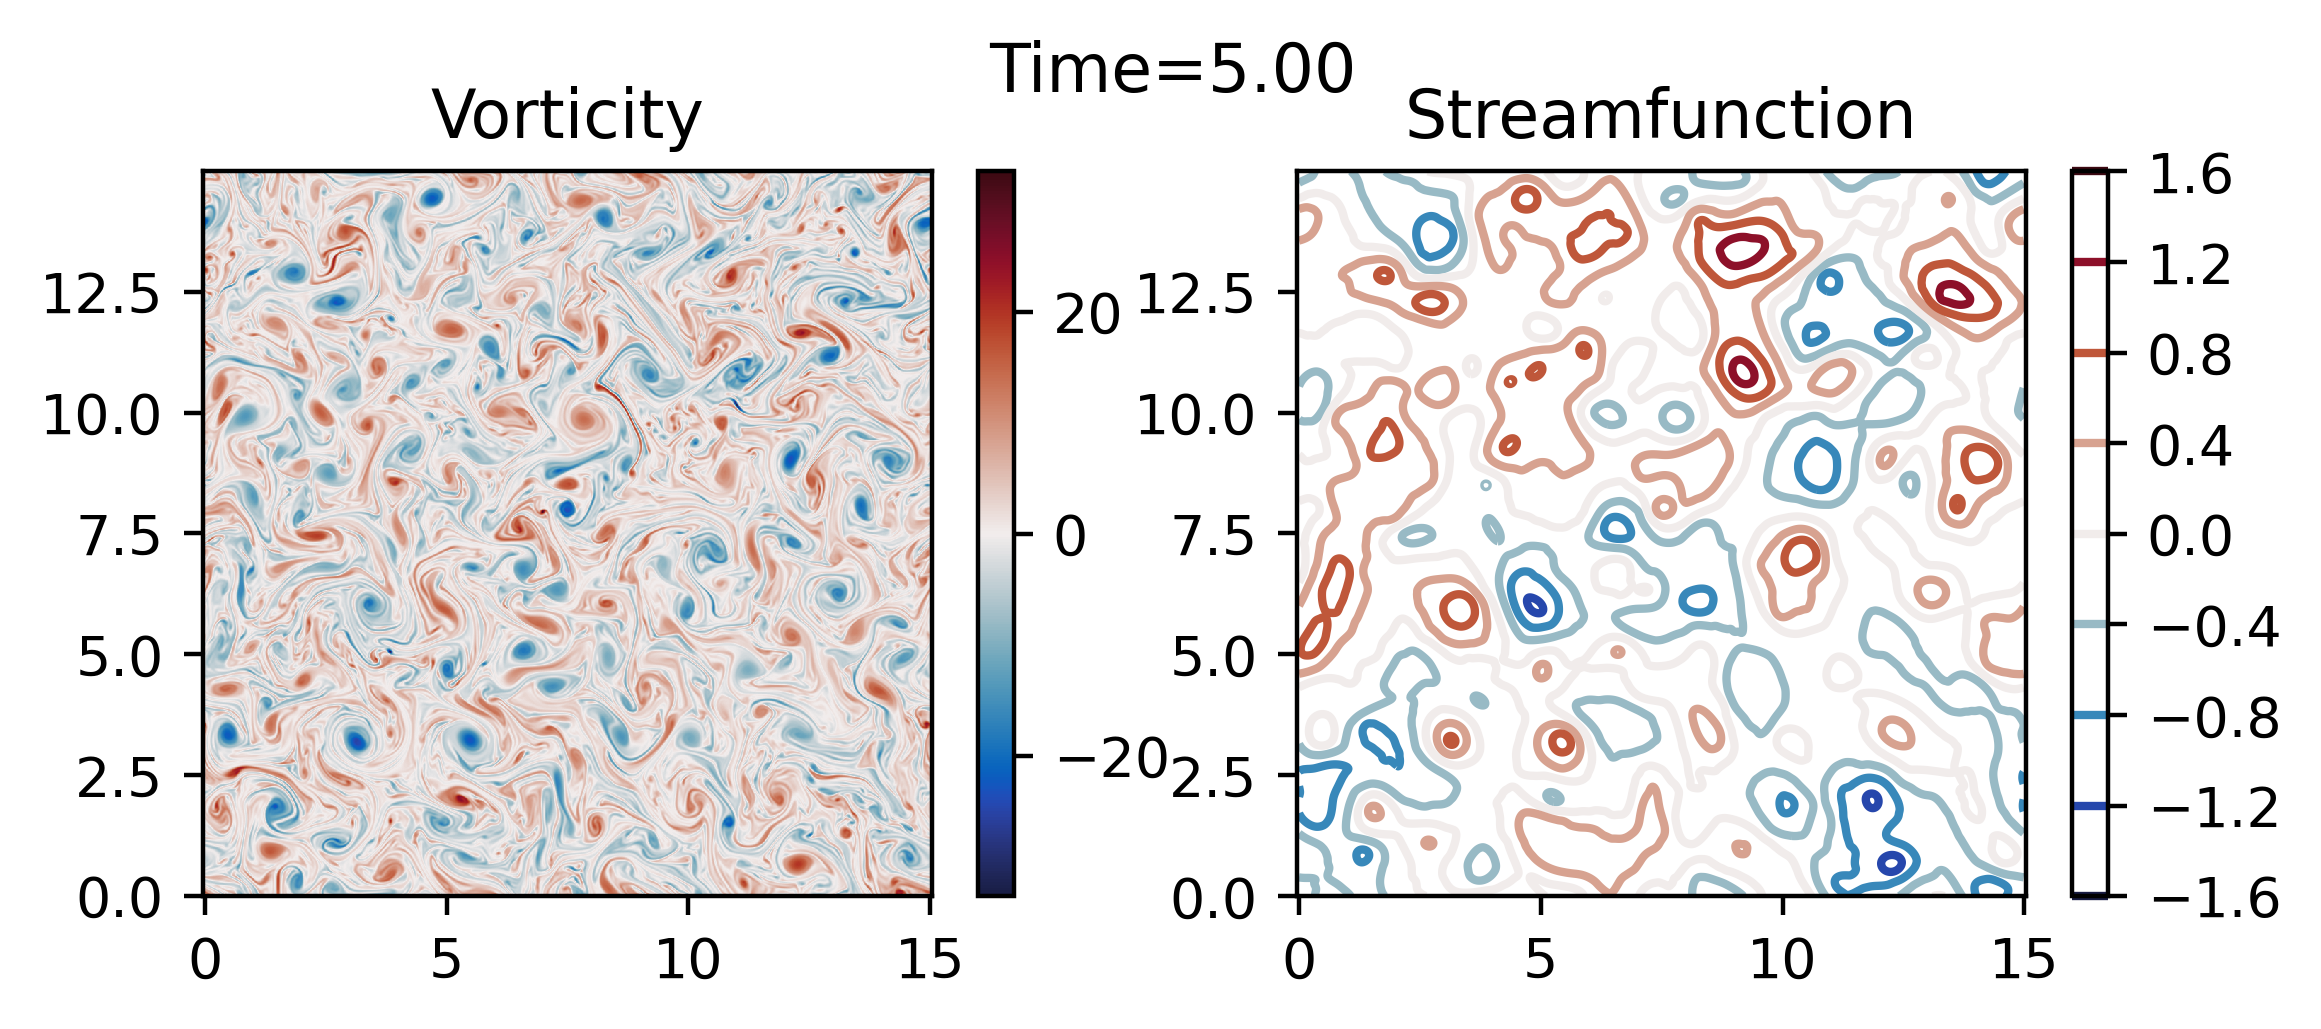
\includegraphics{2DEuler_zeta_t5d00}
    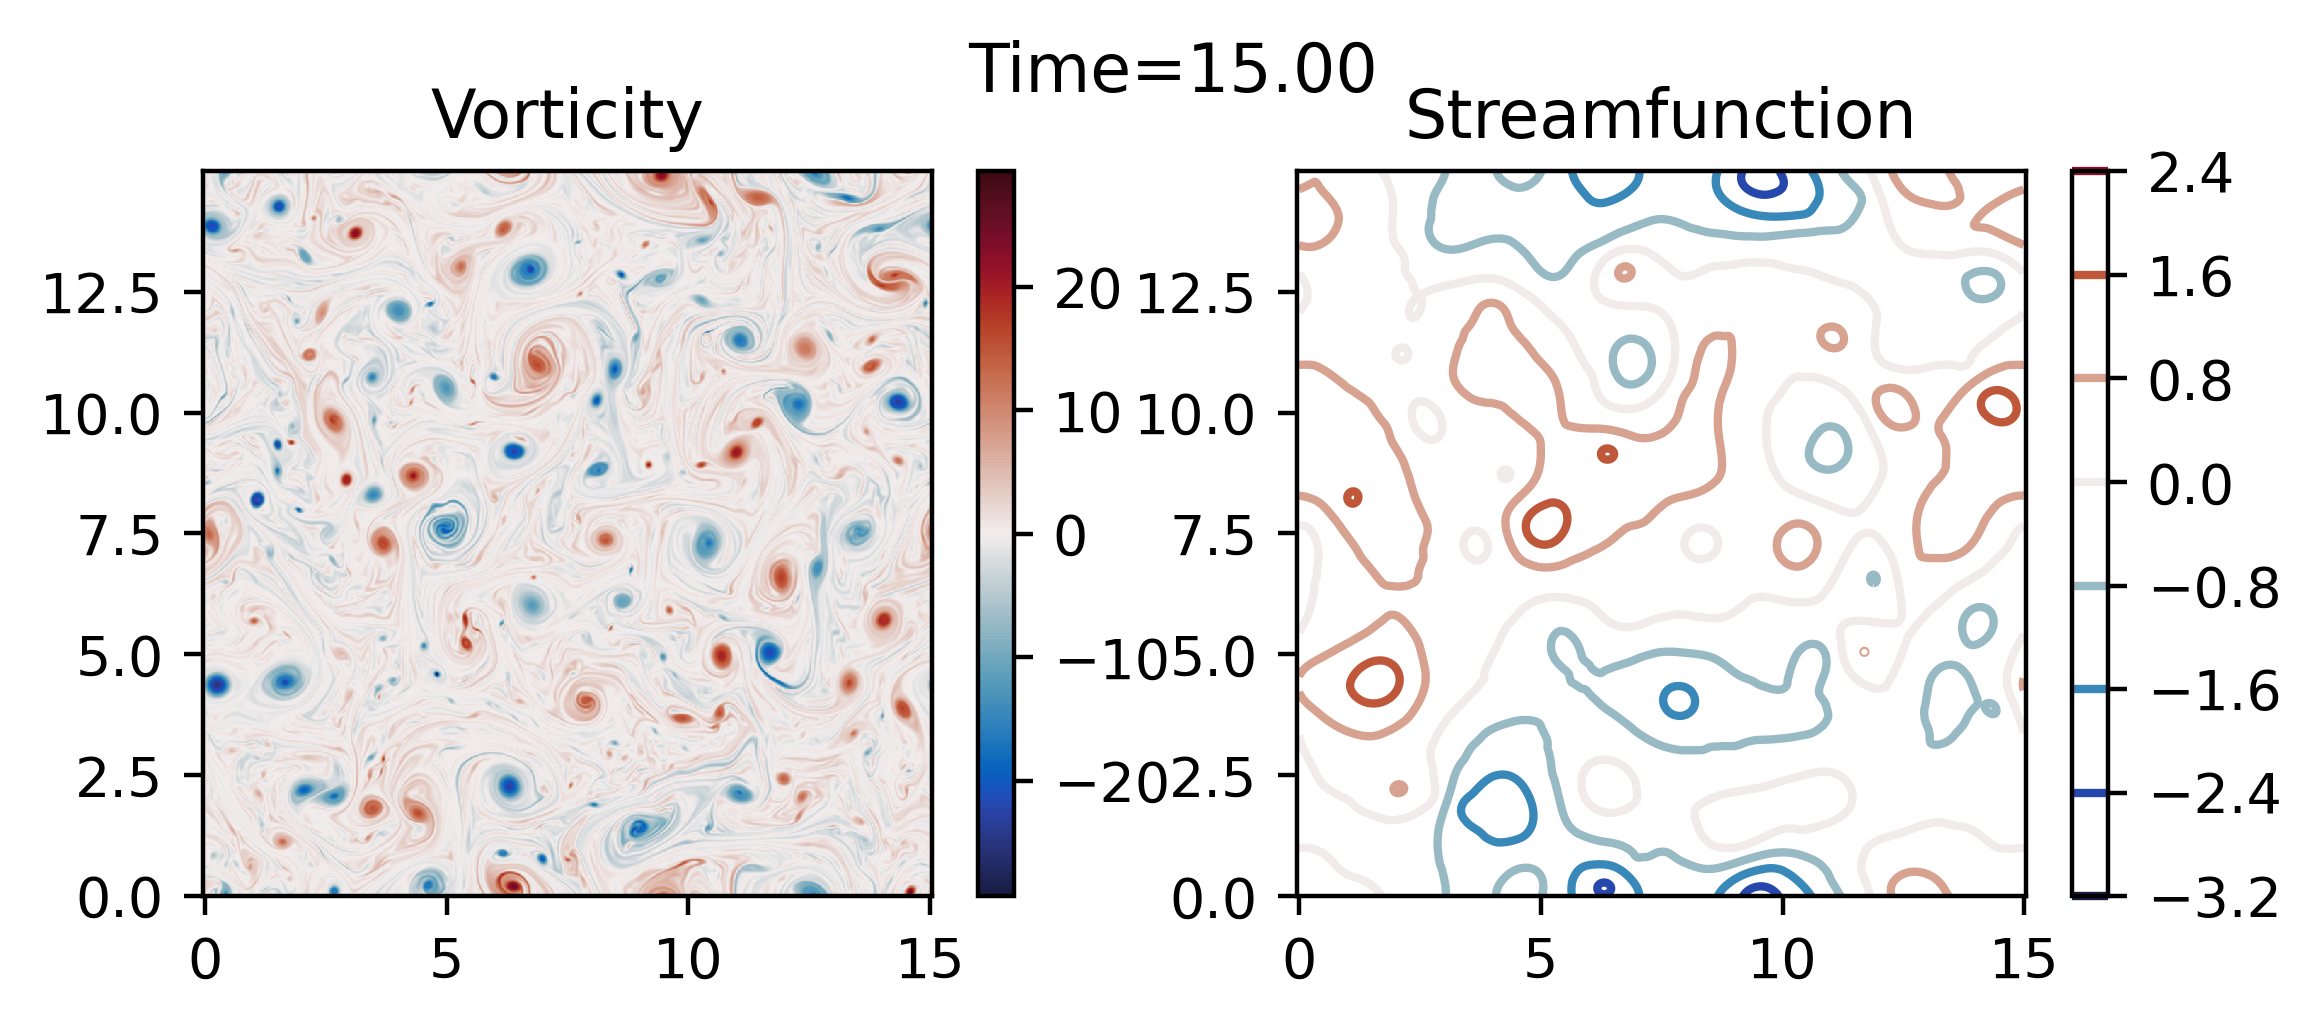
\includegraphics{2DEuler_zeta_t15d00}
    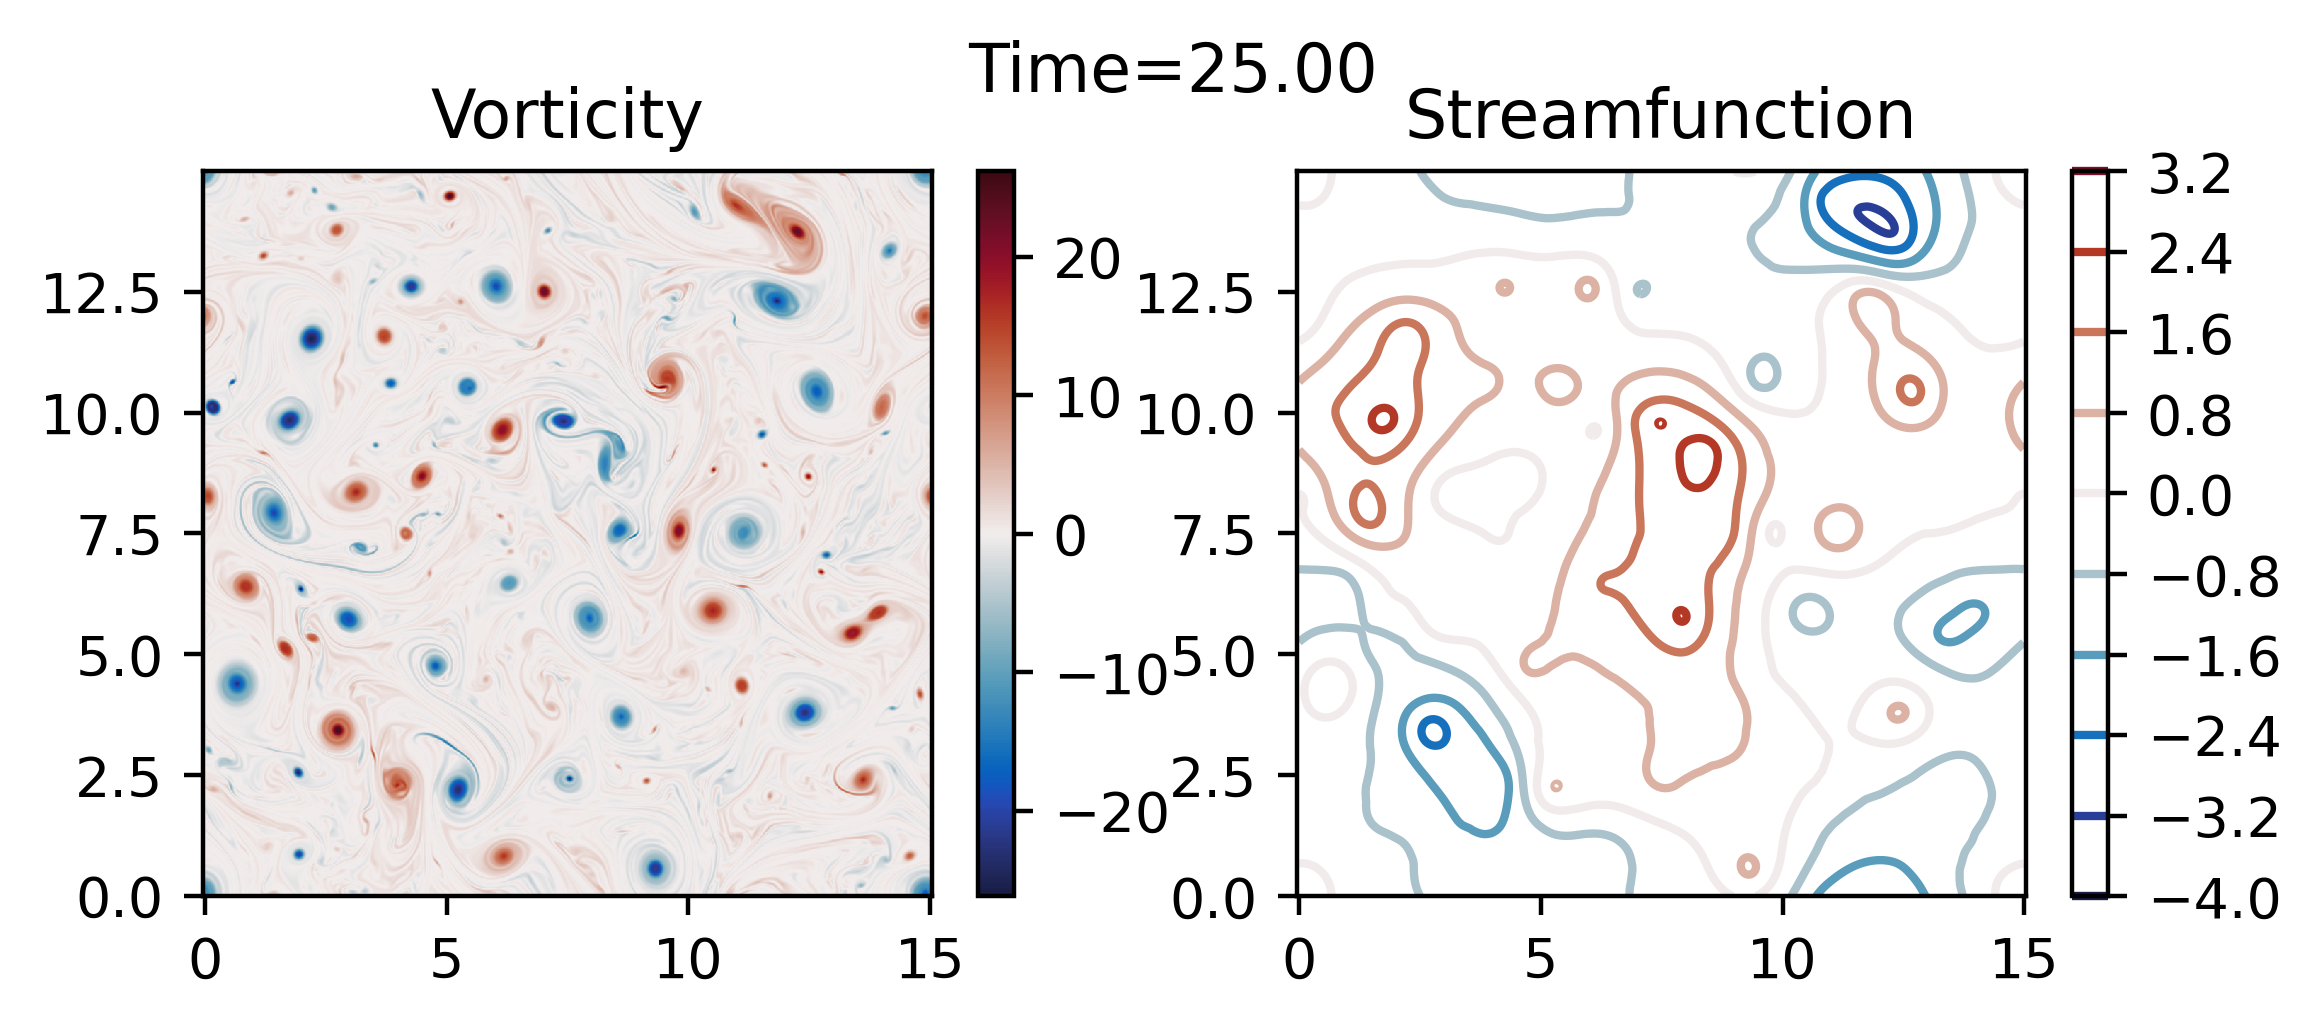
\includegraphics{2DEuler_zeta_t25d00}
    \caption{Snapshots of vorticity and streamfunction 2D Euler simulation overtime.}
    \label{fig:2DEuler_zeta_t}
\end{figure}

\begin{figure}
    \centering
    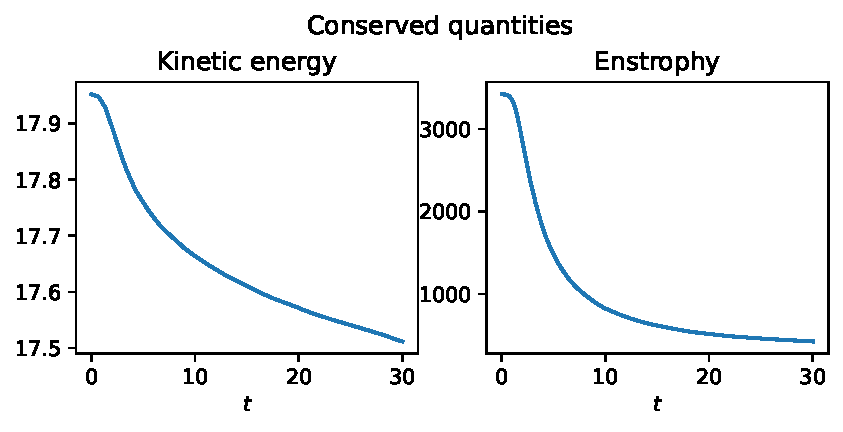
\includegraphics{2DEuler_energy}
    \caption{Time history of kinetic energy and enstrophy of 2D Euler simulation.}
    \label{fig:2DEuler_energy}
\end{figure}

\begin{figure}
    \centering
    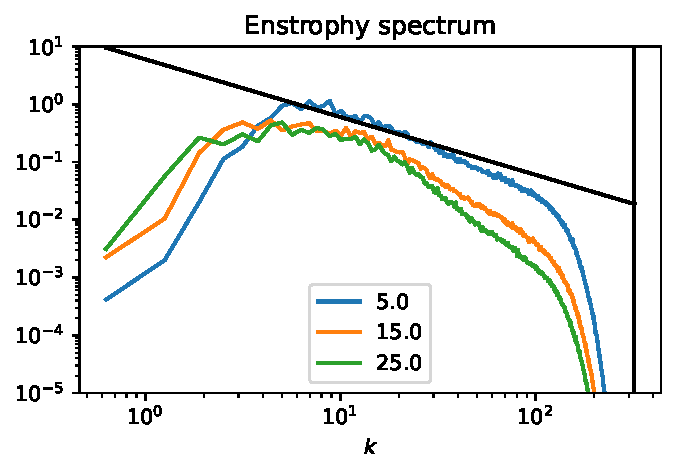
\includegraphics{2DEuler_spec}
    \caption{Time evolution of the enstrophy spectrum of 2D Euler simulation. Legends shows the time. The slanted black line is the $k^{-1}$ reference and the vertical black line is the maximally resolved wavenumber.}
    \label{fig:2DEuler_spec}
\end{figure}

% \section{Vortex crystal on a polar-cap}
% \cite[(2.2.10), p. 603]{Batchelor_53}

\section{Stochastically forced-dissipative simulation}


\section{Wind-forced gyres on a disk}
A particular application of the barotropic vorticity model is the models of wind-forced gyres \cite[\S 19.1.2.I]{Vallis_17}. Dedalus unable to use MPI parallelism when solving equations in a closed box. Therefore we choose to use a disk domain. In some loose sense, it captures the geometry of the Pacific. More importantly, this provides a chance to work with curvilinear domains in Dedalus.

We start with the full nonlinear barotropic vorticity equation on a $\beta$-plane \cite[(19.57)(19.59)]{Vallis_17}, \cite[\S 2]{IerleySheremet_95}:
\begin{align}
    \{R_\beta\}\left[\frac{\pe\zeta}{\pe t}+J(\psi,\zeta)\right]+\beta\frac{\pe\psi}{\pe x} = -\{\epsilon_s\}r\nabla^2\psi+\curl_z\ve\tau_T+\{\epsilon_M\}\nu\nabla^2\psi,
\end{align}
with
\begin{align}
    \psi(r=R) = 0 \qdt{and} \zeta(r=R) = 0.
\end{align}
We have the nondimensional numbers
\begin{align}
    R_\beta &= \frac{|\tau|}{\beta^2R^3};\\
    \epsilon_s &= \frac{r}{R\beta}\\
    \epsilon_M &= \frac{\nu}{\beta R^3}.
\end{align}
where $R$ is the diameter of the circle. 

We pick the 4 gyres wind forcing
\begin{align}
    \curl_z\ve\tau_T = -\sin(4\pi y/R) = -\sin(4\pi r\sin(\theta)/R).
\end{align}


\subsection{The linear Munk model}
We evolve the linear Munk model with $\epsilon_s=0.04$ (cf. \cite[Fig. 19.6]{Vallis_17}) in time till it reaches equilibrium. The model is
\begin{align}
    \beta\frac{\pe\psi}{\pe x}+\{\epsilon_s\}r\nabla^2\psi = \curl_z\ve\tau_T.
\end{align}
We determine that the model has converged by waiting till kinetic energy of the model has stopped changing (not shown) and by visual comparison of the output at different times. Figure \ref{fig:Gyre_stomlin_zetapsi} shows the equilibrated relative vorticity $\zeta$ and streamfunction $\psi$. We see that it looks similar to the Pacific gyres expect our model lack the equatorial dynamics while the real Pacific has the ACC instead of a subpolar gyre in the southern hemisphere.

\begin{figure}
    \centering
    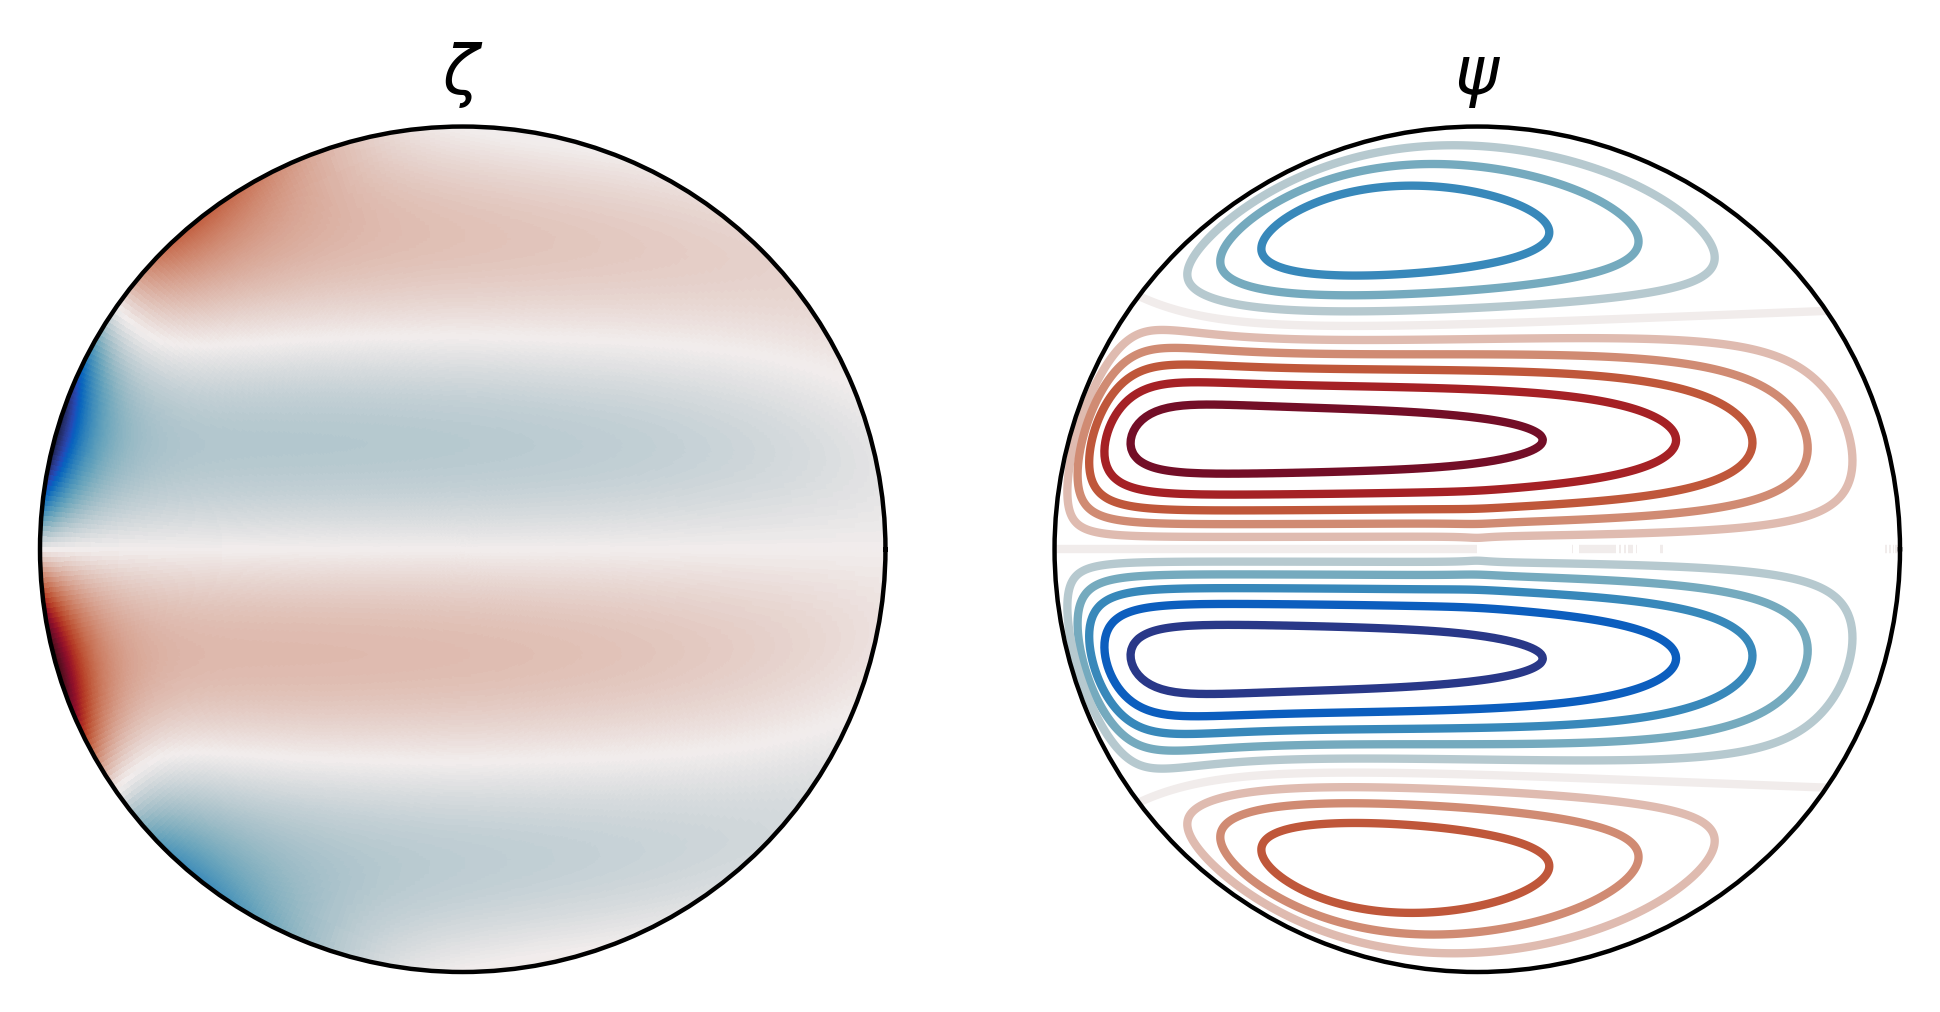
\includegraphics{Gyre_stomlin_zetapsi}
    \caption{Relative vorticity $\zeta$ and streamfunction $\psi$ of the equilibrated linear Munk model.}
    \label{fig:Gyre_stomlin_zetapsi}
\end{figure}

We note that this is a linear boundary value problem and Dedalus has a LBVP module. However, we have not been able to use it for this model because of our implementation of the $\zeta$ term using gradients. A proper solver using the LBVP feature is welcomed.

\subsection{The nonlinear Stommel model}
Now we solve the evolutionary nonlinear Stommel model
\begin{align}
    \{R_\beta\}\left[\frac{\pe\zeta}{\pe t}+J(\psi,\zeta)\right]+\beta\frac{\pe\psi}{\pe x} = \curl_z\ve\tau_T+\{\epsilon_M\}\nu\nabla^2\psi,
\end{align}
with $\epsilon_M = 0.06^3$ (cf. \cite{IerleySheremet_95}) and various value of $R_\beta$ for different nonlinear effects. In particular, the $S=0$ is the linear simulation with the $J(\psi,\zeta)$ term. All simulation has converged to equilibrium according to the the above definition. Figure \ref{fig:Gyre_munk_zetaall} shows the streamfunctions for simulation with different nonlinearities, titled by $S = \sqrt{R_\beta}$. This resembles the Munk (slip) case of \cite[Fig. 19.11]{Vallis_17}. We see that more stronger advection would push the circulation pattern towards the direction of the flow, eventually separating the subtropical gyres into two smaller ones. We also see the more nonlinear simulation has less pronounced western boundary currents. This is consistent with the results of \cite[Fig. 19.11]{Vallis_17} and \cite[Figure 2]{IerleySheremet_95}.

It is known that the nonlinear Munk model has multiple stable equilibriums in certain parameter regimes \parencite{CessiIerley_95, IerleySheremet_95}. Our time evolution method could be adapted to change the parameters slowly (via restarting) to find the equilibriums. We do not pursue that direction here any further.

\begin{figure}
    \centering
    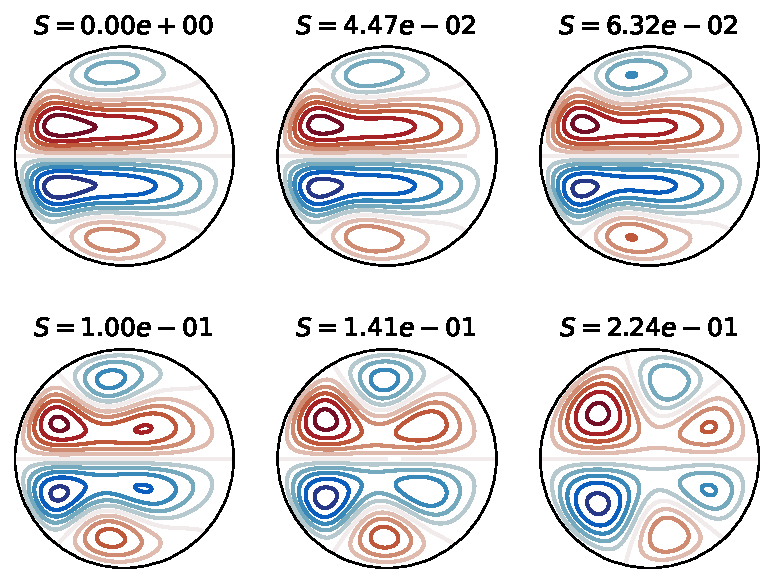
\includegraphics{Gyre_munk_zetaall}
    \caption{Streamfunctiona $\psi$ of the equilibrated nonlinear Munk model titled by $S = \sqrt{R_\beta}$}
    \label{fig:Gyre_munk_zetaall}
\end{figure}

% \chapter{2D Barotropic Quasi-geostrophic (QG) model}
% \cftchapterprecis{Ryan Sh\`iji\'e D\`u}
% \graphicspath{{QG/code/}}
\renewcommand{\Bu}{\text{Bu}}
\renewcommand{\Ub}{\text{Bu}^{-1}}

\section{Barotropic QG model}
We have
\begin{align}
    &\frac{\DD}{\DD t} q+\{\xi^{-2}\}\beta v = 0,\\
    &q = \nabla^2\psi - \{\Bu^{-1}\} k_d^2\psi,\\
    &u = -\frac{\pe\psi}{\pe y}, v = \frac{\pe\psi}{\pe x}.
\end{align}
where the 
\begin{align}
    \xi^{-2} = \frac{\beta L^2}{U} \qdt{,} \text{Bu} = \frac{gH}{f_0^2L^2} = \frac{L_{d}^2}{L^2}
\end{align}

\subsection{Nonlinear freely decaying simulation}
This is an easy modification of the barotropic vorticity code.

\subsection{Rossby wave}
We simulate finite deformation radius Rossby waves in a circle gyre. There is no mean flow $U$ in this example. We use the linear barotropic QG model. That is, we use \parencite[(6.64)]{Vallis_17}:
\begin{align}
    &\frac{\pe}{\pe t} q+\{\xi^{-2}\}\beta v = 0,\\
    &q = \nabla^2\psi - \{\Bu^{-1}\} k_d^2\psi,\\
    &u = -\frac{\pe\psi}{\pe y}, v = \frac{\pe\psi}{\pe x}.
\end{align}
Standard derivation gives the dispersion relation for this Rossby wave \parencite[(RW.3)]{Vallis_17}:
\begin{align}
    \omega = \frac{-\{\xi^{-2}\}\beta k}{k^2+\ell^2+\{\Bu^{-1}\}k_d^2}
\end{align}
We then have the phase velocity in the $x$-direction is
\begin{align}
    c_p^x = \frac{\omega\cdot k}{(k^2+\ell^2)} = \frac{-\{\xi^{-2}\}\beta k^2}{(k^2+\ell^2+\{\Bu^{-1}\}k_d^2)(k^2+\ell^2)}<0.
\end{align}
The group velocity is \parencite[(RW.4)]{Vallis_17}
\begin{align}
    c_g^x = \frac{\pe\omega}{\pe k} = \frac{\{\xi^{-2}\}\beta(k^2-\ell^2-\{\Bu^{-1}\}k_d^2)}{(k^2+\ell^2+\{\Bu^{-1}\}k_d^2)}.
\end{align}
We see that the phase velocity of the Rossby wave is always westward ($\beta>0$ always), while the group velocity's direction depends on the spatial scale of the wave.

We simulate Rossby waves with $\Bu=1$ an $\xi^{-2}=1$ to focus on the effects of wave size. First, we make a wave package with $k=0.7$ and $\ell=0$. We plot the wave after some time in Figure \ref{fig:Rossby_k0d7_tt20d11}. It is clear that the group velocity is westward because the package has moved west. To see that the phase velocity is westward, please watch the \href{https://vimeo.com/936333986}{video}. 

\begin{figure}
    \centering
    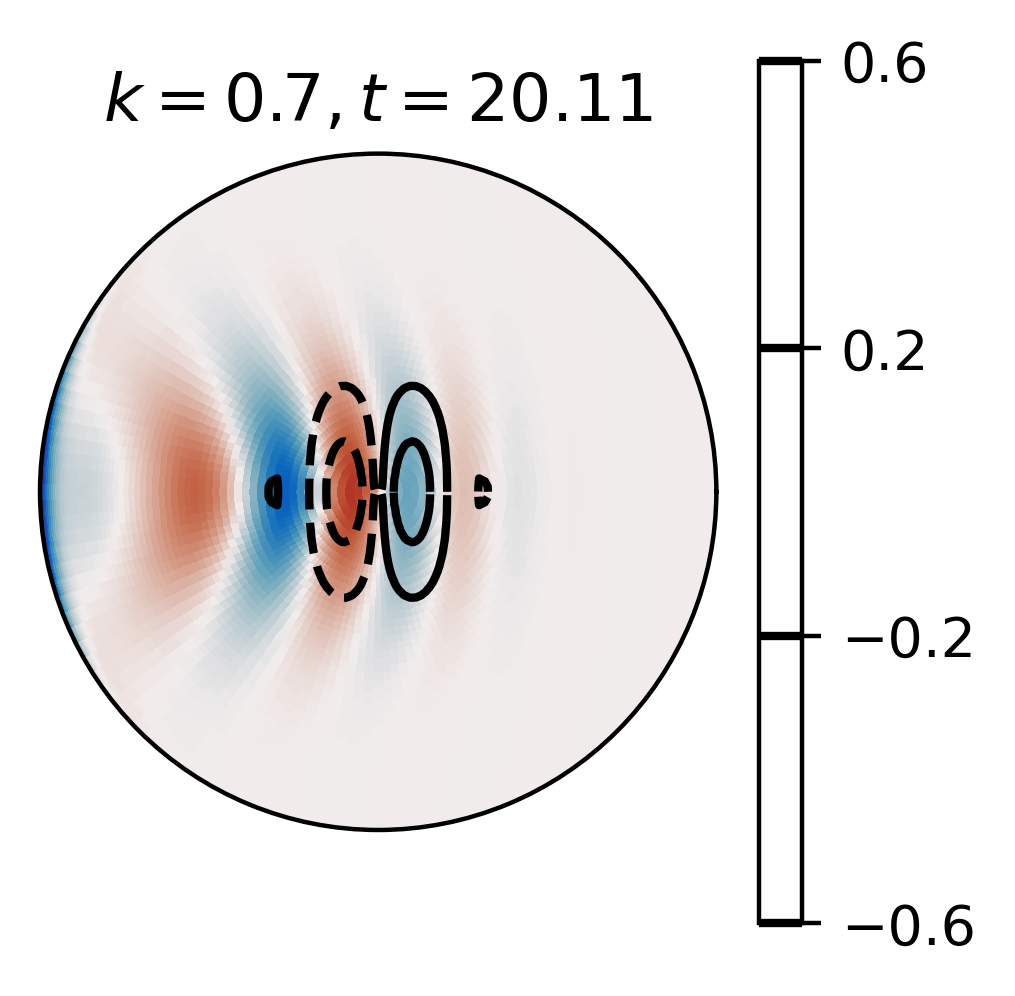
\includegraphics{Rossby_plots/Rossby_k0d7_tt20d11}
    \caption{}
    \label{fig:Rossby_k0d7_tt20d11}
\end{figure}

\href{https://vimeo.com/936333886}{video}. 


% \section{The full model nondimensionalized}
% We start with the 2 layer QG model with mean flow, $\beta$, and topography \parencite[(5.85-86)]{Vallis_17} (in the notation of \cite{Vallis_96a}):
% \begin{align}
%     &\frac{\pe q_1}{\pe t}+J(\psi_1,q_1)+U_1\frac{\pe q_1}{\pe x}+\left(\{\xi_1^{-2}\}\beta+\{\Bu_1^{-1}\}\frac{f_0^2(U_1-\{U_r\}U_2)}{g'H_1}\right)\frac{\pe\psi_1}{\pe x} = 0;\label{eq:2lay_eq1}\\
%     \{A\}&\frac{\pe q_2}{\pe t}+J(\psi_2,q_2)+U_2\frac{\pe q_2}{\pe x}+\left(\{\xi_2^{-2}\}\beta+\{\Bu_2^{-1}\}\frac{f_0^2(U_2-\{U_r^{-1}\}U_1)}{g'H_2}\right)\frac{\pe\psi_2}{\pe x} = 0.\label{eq:2lay_eq2}
% \end{align}
% where
% \begin{align}
%     q_1 &= \nabla^2\psi_1 + \{\Bu_1^{-1}\}\frac{f_0^2}{g'H_1}(\{U_r\}\psi_2-\psi_1);\label{eq:2lay_pv1}\\
%     q_2 &= \nabla^2\psi_2 + \{\Bu_2^{-1}\}\frac{f_0^2}{g'H_2}(\{U_r^{-1}\}\psi_1-\psi_2)+\left\{\frac{\alpha}{\text{Ro}_2}\right\}\frac{f_0}{H_2}\eta.\label{eq:2lay_pv2}
% \end{align}
% We have nondimensionalized time to be the advective timescale of the first layer:
% \begin{align}
%     T = \frac{L_1}{U_1}.
% \end{align}
% Then we nondimensionalized \eqref{eq:2lay_eq1} and \eqref{eq:2lay_pv1} with length $L_1$ and \eqref{eq:2lay_eq2} and \eqref{eq:2lay_pv2} with length $L_2$. We have introduced the nondimensional number $\xi$ which is the ratio between the Rhine scale and the lengthscale of each layer \parencite{HeldLarichev_96}
% \begin{align}
%     \xi_i^{-2} = \frac{\beta L_i^2}{|U_i|}
% \end{align}
% and $\alpha$ which is the ratio of the typical topographic height versus the second layer's height
% \begin{align}
%     \alpha = \frac{\eta}{H_2}.
% \end{align}
% If the height and mean flow of the two layers are not equal, we have two parameters for their ratio
% \begin{align}
%     U_r = \frac{|U_2|}{|U_1|}, \qdt{and} A = \frac{|U_1|L_2}{|U_2|L_1}
% \end{align}
% We also have the more familiar quantities
% \begin{align}
%     L_{i,d} = \frac{\sqrt{g'H_i}}{f_0} \qdt{,} \text{Ro}_2 = \frac{|U_2|}{f_0L_2} \qdt{and} \text{Bu}_i = \frac{L_{i,d}^2}{L_i^2}.
% \end{align}

\section{The 2-layer QG model under Phillips baroclinic instability}
\subsection{The nondimensional equations}
The 2-layer model simplifies drastically when we make the upper/lower layer symmetry assumption \parencite{LarichevHeld_95}. We take $H_1=H_2 = H/2$ and $U_1=-U_2=U$. Then the equation becomes
\begin{align}
    &\frac{\pe q_1}{\pe t}+J(\psi_1,q_1)+U\frac{\pe q_1}{\pe x}+\left(\{\xi^{-2}\}\beta+\{8\Bu^{-1}\}\frac{4f_0^2U}{g'H}\right)\frac{\pe\psi_1}{\pe x} = 0,\label{eq:2lay_sym_eq1}\\
    &\frac{\pe q_2}{\pe t}+J(\psi_2,q_2)-U\frac{\pe q_2}{\pe x}+\left(\{\xi^{-2}\}\beta-\{8\Bu^{-1}\}\frac{4f_0^2U}{g'H}\right)\frac{\pe\psi_2}{\pe x} = 0;\label{eq:2lay_sym_eq2}
\end{align}
where
\begin{align}
    q_1 &= \nabla^2\psi_1 + \{4\Bu^{-1}\}\frac{2f_0^2}{g'H}(\psi_2-\psi_1),\label{eq:2lay_sym_pv1}\\
    q_2 &= \nabla^2\psi_2 + \{4\Bu^{-1}\}\frac{2f_0^2}{g'H}(\psi_1-\psi_2)+\left\{\frac{\alpha}{\text{Ro}}\right\}\frac{2f_0}{H}\eta.\label{eq:2lay_sym_pv2}
\end{align}
We have 
\begin{align}
    \xi^{-2} = \frac{\beta L^2}{U} \qdt{,} \text{Bu} = \frac{2g'H}{f_0^2L^2} = \frac{L_{d}^2}{L^2} \qdt{and} \alpha = \frac{2\eta}{H}.
\end{align}
Note that this implies (cf. \cite[(9.103)]{Vallis_17})
\begin{align}
    L_d = \frac{2\sqrt{g'H/2}}{f_0} \qdt{with} k_d^2 = \frac{4f_0^2}{g'H} = \frac{8}{L_d^2}.
\end{align}
This is an ok definition when we connect to the continuously stratified case by using (cf. \cite[(5.138)]{Vallis_17})
\begin{align}
    L_d = \frac{NH}{f} \qdt{with} N^2 = \frac{g'}{H/2}.
\end{align}
$\xi$ and $\Bu$ are not independent since their only freedom is in picking $L$. In our simulation, we pick $L=L_d$ such that $\text{Bu}=1$. 
We further simplify by setting flat topography ($\alpha=0$). The only free parameter is $\xi$
\begin{align}
    \xi^{-2}= \frac{\beta L^2}{U} = \frac{\beta L_d^2}{U}
\end{align}
It is the two-layer version of the `Charney–Green number’. 

Finally, we simulate using a $|k|^8$ hyper-diffusivity on $q_i$ for small scale dissipation and an Ekman damping only in the bottom layer for damping the inverse cascade.

\subsection{Linear stability analysis}
We take only the linear terms of the above model, and dispense of all unnecessary parameters:
\begin{align}
    &\frac{\pe q_1}{\pe t}+\frac{\pe q_1}{\pe x}+\left(\xi^{-2}+8\Bu^{-1}\right)\frac{\pe\psi_1}{\pe x} = 0,\label{eq:2lay_sym_eq1_lin}\\
    &\frac{\pe q_2}{\pe t}-\frac{\pe q_2}{\pe x}+\left(\xi^{-2}-8\Bu^{-1}\right)\frac{\pe\psi_2}{\pe x} = 0;\label{eq:2lay_sym_eq2_lin}
\end{align}
where
\begin{align}
    q_1 &= \nabla^2\psi_1 + 4\Bu^{-1}(\psi_2-\psi_1),\label{eq:2lay_sym_pv1_lin}\\
    q_2 &= \nabla^2\psi_2 + 4\Bu^{-1}(\psi_1-\psi_2).\label{eq:2lay_sym_pv2_lin}
\end{align}

This system if isomorphic to \cite[(9.107)]{Vallis_17}. Therefore we can copy down the answer:
\begin{align}
    c &= -\frac{\xi^{-2}}{K^2+8\Bu^{-1}}\left\{ 1+\frac{8\Bu^{-1}}{2K^2}\pm\frac{8\Bu^{-1}}{2K^2}\left[1+4\frac{K^4(K^4-8^2\Bu^{-2})}{8^2\xi^{-4}\Bu^{-2}}\right]^{1/2} \right\}.
\end{align}
We have recovered \cite[(9.114)]{Vallis_17} with $\hat{k}_d^2 = 8$ and (cf. \cite[(9.115)]{Vallis_17})
\begin{align}
    \xi^{-2} = \hat{k}_\beta^2 = \frac{\beta L_d^2}{U}.
\end{align}

Now we can use the eigenvalue-problem module of Dedalus is solve the same problem numerically. Figure \ref{fig:2Lay_linstab} shows the growth rate. This is a reproduction of \cite[Fig. 9.14]{Vallis_17}.
\begin{figure}
    \centering
    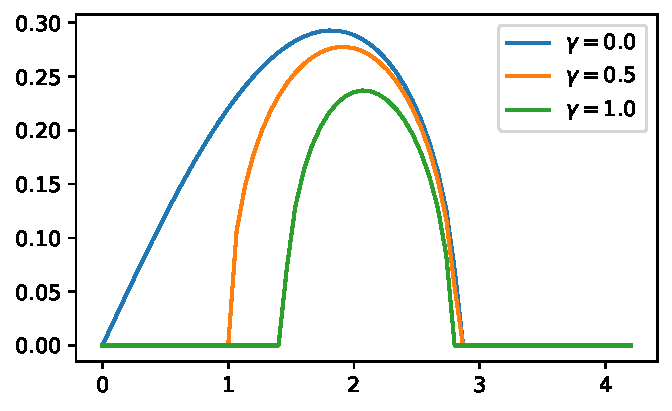
\includegraphics{plot_snap/figs/2Lay_linstab}
    \caption{}
    \label{fig:2Lay_linstab}
\end{figure}


\subsection{Simulation of jets formation}
We pick $\xi = 0.4$ for a large $\zeta$ effect while still having a baroclinically unstable background. At early times, baroclinic instability appears with its distinct pattern. In Figure \ref{fig:2Layjets_q1_t6d50} we also plot a sin wave with $2.26$ wavenumber, the fastest growing mode for $\xi = 0.4$. We see that the instability pattern matches the theory. At later times, the flow develops into jets. Figure \ref{fig:2Layjets_q1_t150d00} shows clear PV staircases with homogenized regions in between. Figure \ref{fig:2Layjets_q1zonalmean_t150d00} plots the zonally averaged perturbation PV $q_1$ against a sin wave of wavenumber $1/2\xi$. We see that matches well the distance between jets. Note that
\begin{align}
    \frac{1}{2\xi} = \frac{1}{2}\hat{k}_\beta = \sqrt{\gamma}
\end{align}
where $\gamma$ is defined in \cite[(9.115)]{Vallis_17}. 

\begin{figure}
    \centering
    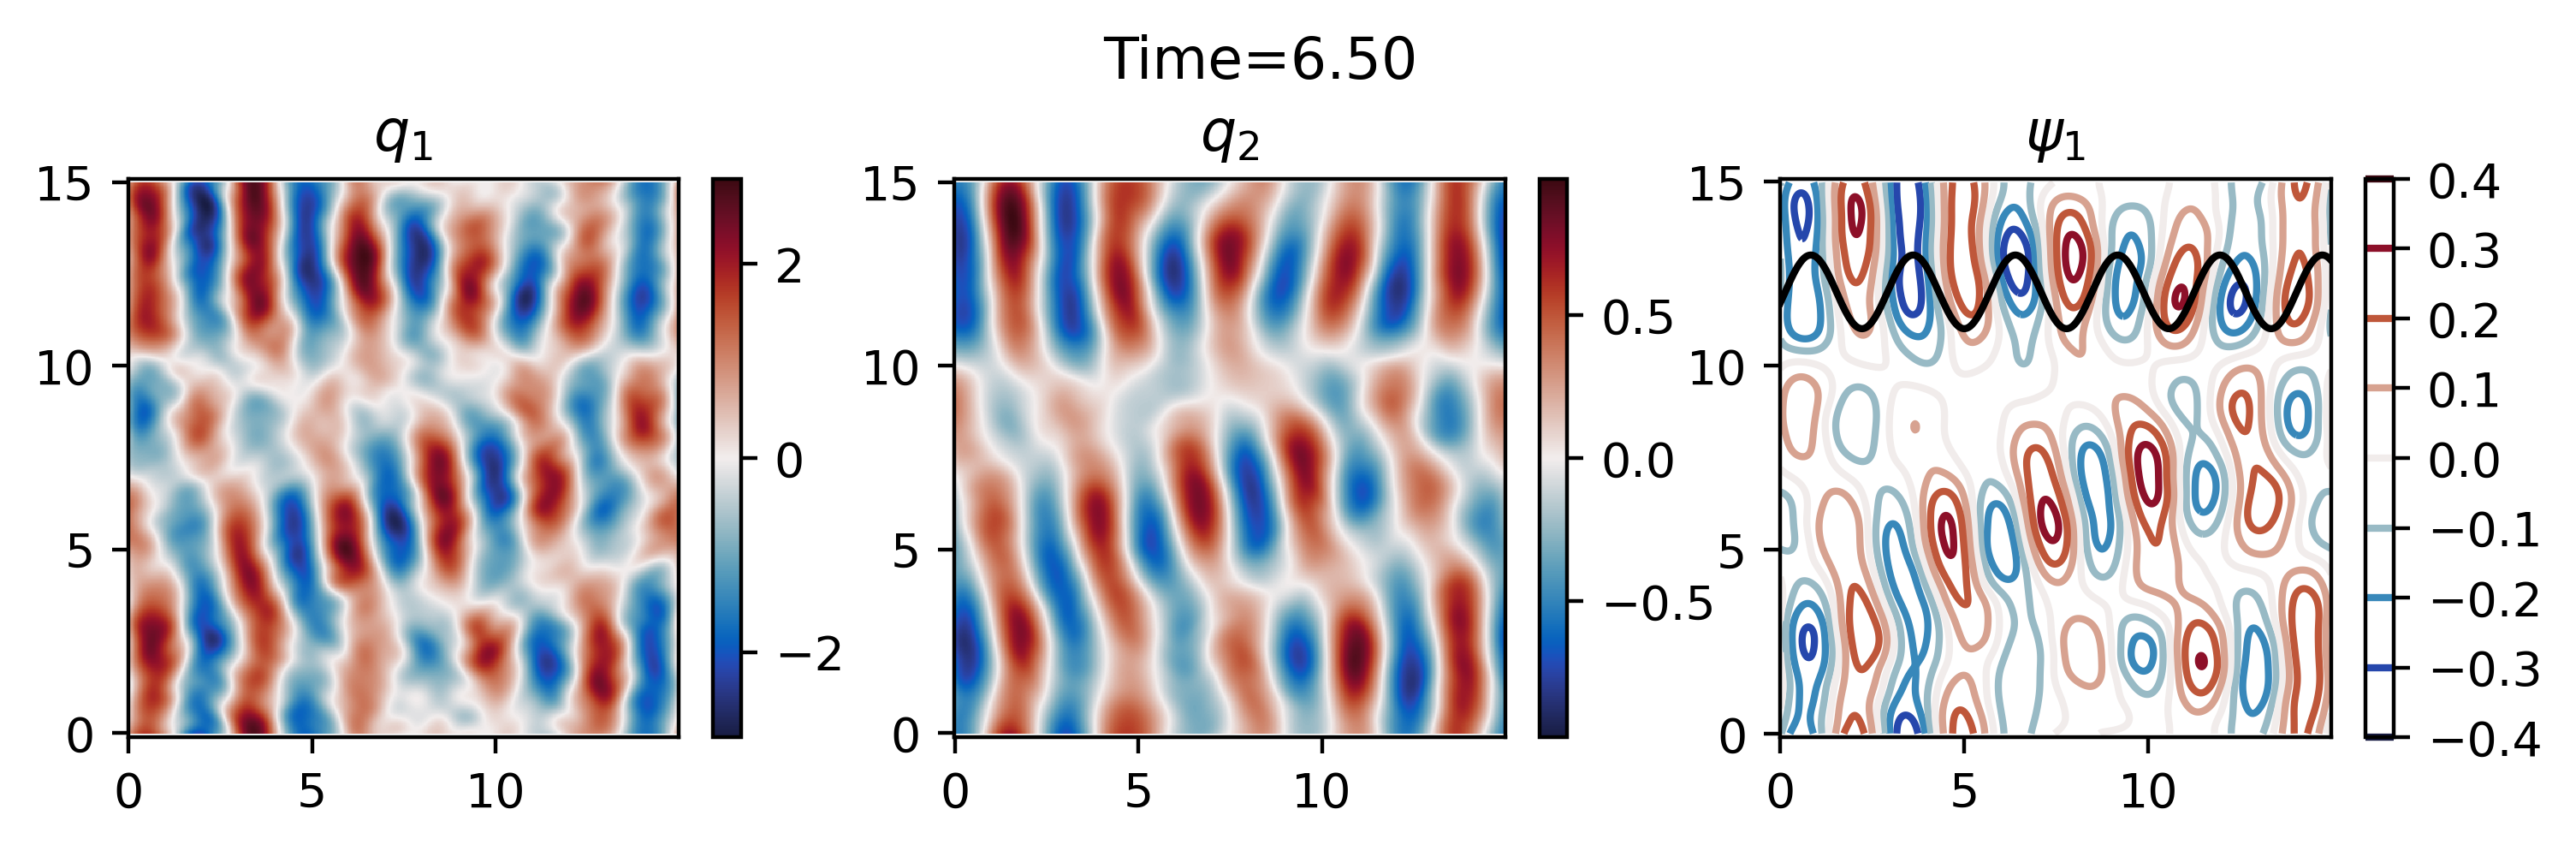
\includegraphics[width=\textwidth]{plot_snap/figs/2Layjets_q1_t6d50}
    \caption{}
    \label{fig:2Layjets_q1_t6d50}
\end{figure}


\begin{figure}
    \centering
    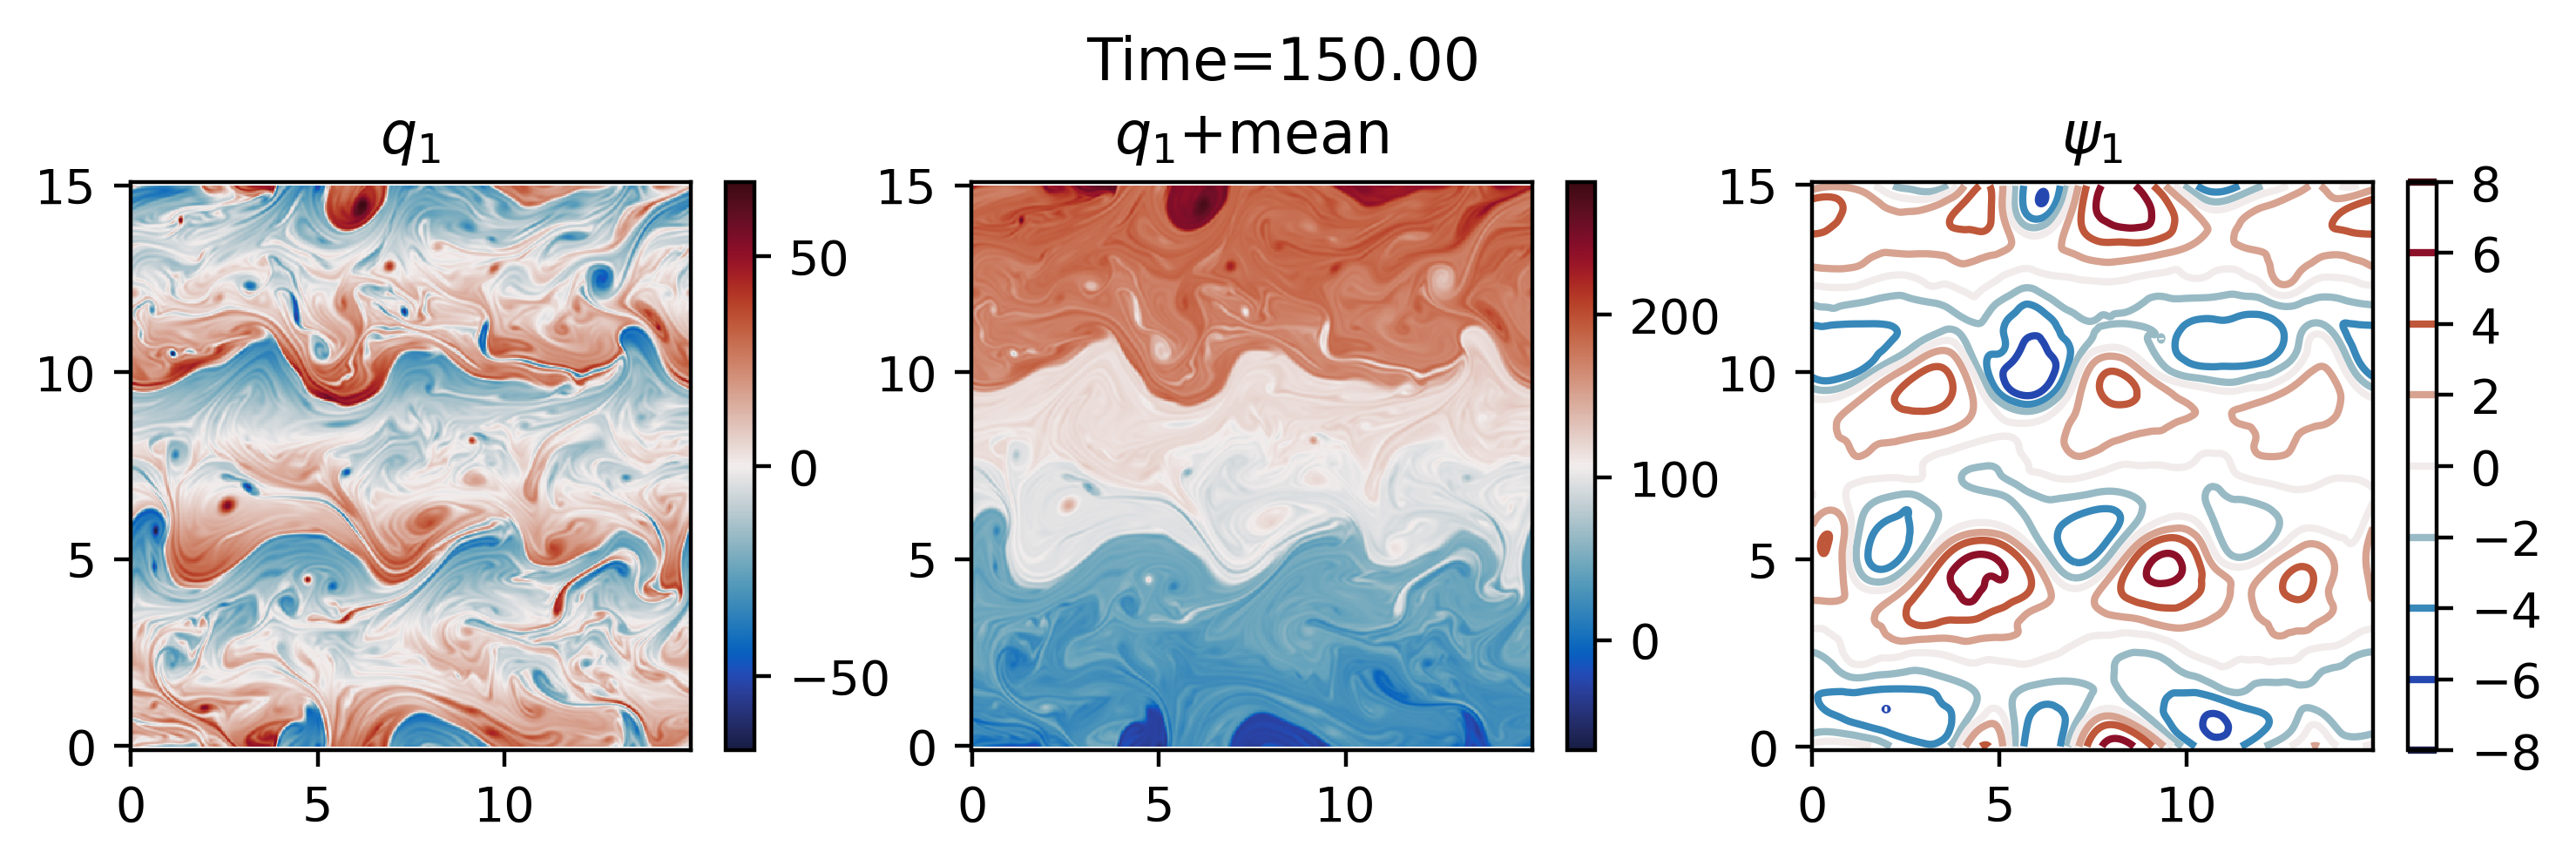
\includegraphics[width=\textwidth]{plot_snap/figs/2Layjets_q1_t150d00}
    \caption{}
    \label{fig:2Layjets_q1_t150d00}
\end{figure}

\begin{figure}
    \centering
    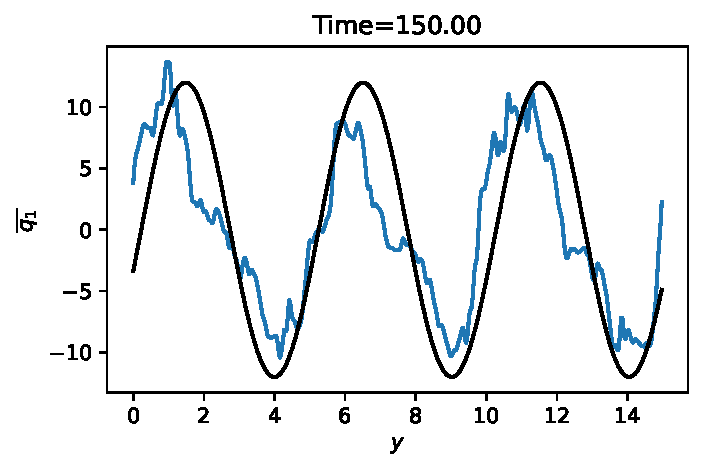
\includegraphics{2Layjets_q1zonalmean_t150d00}
    \caption{}
    \label{fig:2Layjets_q1zonalmean_t150d00}
\end{figure}

\subsection{2 layer turbulence}
We instead pick $\xi=1.5$ on a larger domain for a simulation with small $\beta$ effect. Figure \ref{fig:2Lay_qbrbc_t150d00} shows the barotropic and baroclinic PV. These are visually similar to \cite[Fig. 3]{LarichevHeld_95}. We also plot the $q_1$ enstrophy spectrum in Figure \ref{fig:2Lay_q1spec_t150d00}. The spectrum has a slope of $-1$, matching the theoretical expectation.

\begin{figure}
    \centering
    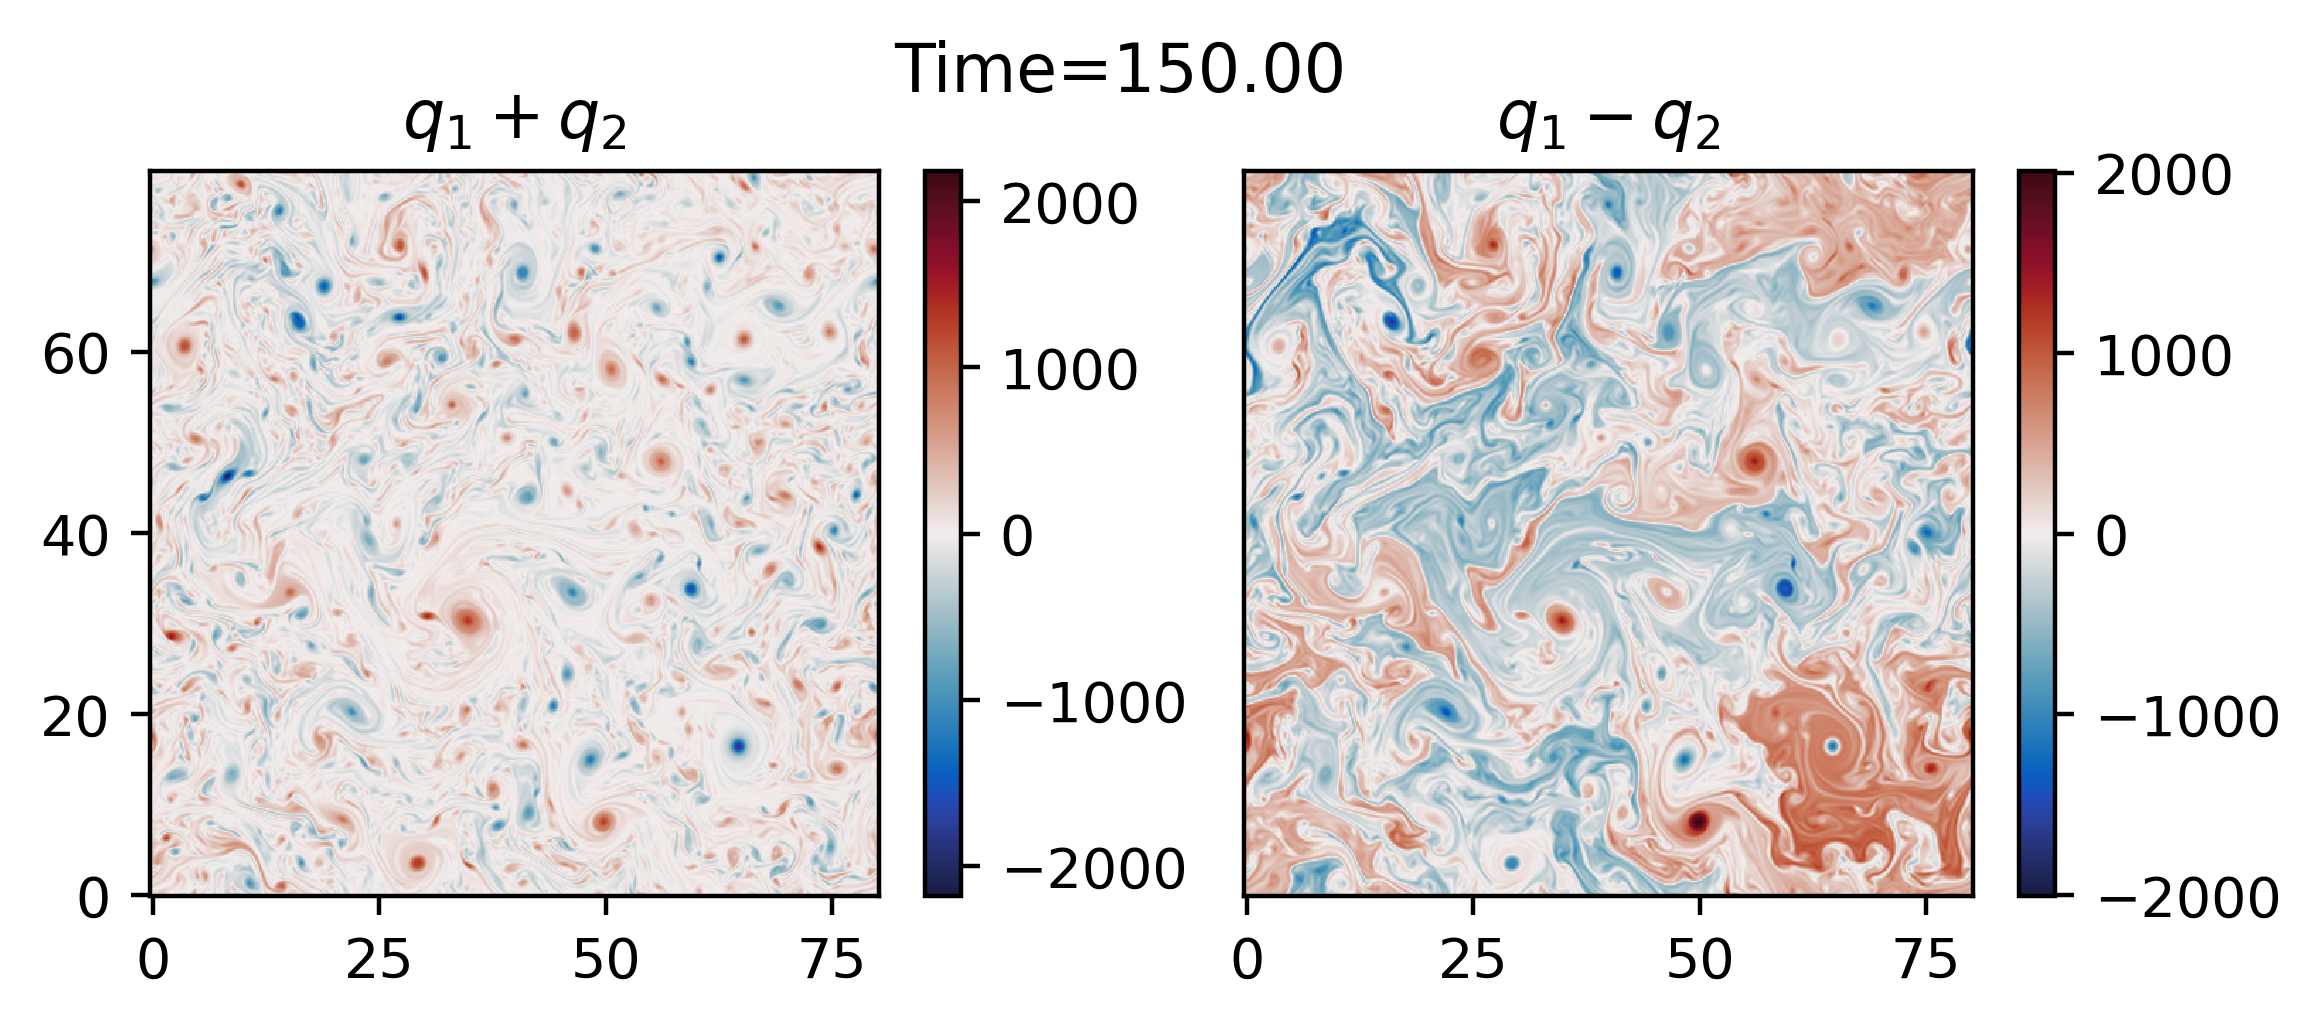
\includegraphics{plot_snap/figs/2Lay_qbrbc_t150d00}
    \caption{}
    \label{fig:2Lay_qbrbc_t150d00}
\end{figure}

\begin{figure}
    \centering
    
\includegraphics{plot_snap/figs/2Lay_q1spec_t150d00}
    \caption{}
    \label{fig:2Lay_q1spec_t150d00}
\end{figure}

\chapter{2D QG-Near Inertial Wave (QG-NIW) model}
\cftchapterprecis{Ryan Sh\`iji\'e D\`u}
\graphicspath{{2D_QGNIW/figs/}}

The QG-NIW model was derived in \cite{XieVanneste_15}. It has been since further explored and expanded by \cite{WagnerYoung_15, WagnerYoung_16, AsselinYoung_19} and others. Here we will implement the two-dimensional version in \cite{RochaEtAl_18}. 

\section{The QG-NIW model}
We have the dimensional QG-NIW model (ignoring dissipation) from \cite[(2.6--8)]{RochaEtAl_18}:
\begin{align}
    &q = \nabla^2\psi + \frac{1}{f}\left[\frac{1}{4}\nabla^2|\phi|^2+\frac{i}{2}J(\phi^*,\phi)\right];\\
    &q_t + J(\psi,q) = 0;\\
    &\phi_t+J(\psi,\phi)+\phi\frac{i}{2}\nabla^2\psi-\frac{i}{2} \frac{N^2}{f m^2} \nabla^2\phi = 0.
\end{align}

\subsection{Nondimensionalization}
We make clear the true parameters dependence of the model by nondimensionalizing the model with:
\begin{align}
    &\phi \sim U_w = \epsilon^{-1} U_e\\
    &\psi \sim U_e L\\
    &L \sim L_e = k_e^{-1}\\
    &T \sim L/U_e
\end{align}
where
\begin{align}
    \epsilon = {U_e}/{U_w}\ll 1
\end{align}
indicated we are in the weak wave regime. Then we get (in the notation of \cite{Vallis_96a}):
\begin{align}
    &q = \nabla^2\psi + \frac{1}{f}\{\alpha\}\left[\frac{1}{4}\nabla^2|\phi|^2+\frac{i}{2}J(\phi^*,\phi)\right];\\
    &q_t + J(\psi,q) = 0;\\
    &\phi_t+J(\psi,\phi)+\phi\frac{i}{2}\nabla^2\psi-\frac{i}{2} \frac{N^2}{f m^2} \{\hbar\}\nabla^2\phi = 0\label{eq:QGNIW_eq3}
\end{align}
where we have the model depends on only two important nondimensional numbers, the wave amplitude:
\begin{align}
    &\alpha = \frac{U_e}{fL}\epsilon^{-2} = \text{Ro}\;\epsilon^{-2},
\end{align}
and the wave dispersivity:
\begin{align}
    &\hbar = \frac{N^2}{fm^2}\frac{1}{LU_e} = \frac{1}{\text{Ro}}\frac{N^2}{f^2 m^2 L^2}.
\end{align}
Note that Rossby number and the small parameter $\epsilon$ does not appear explicitly in the model. We only assume that they are small. Instead, their ratio appear as the wave amplitude $\alpha$. The distinguished limit assumptions in \cite{XieVanneste_15, WagnerYoung_15, WagnerYoung_16} is $\alpha = 1$. However, in \cite{RochaEtAl_18} it is allowed to vary in the $O(1)$ range. We also noticed that the Rossby number in \cite[Table 4]{RochaEtAl_18} is wrong. It should be $\approx 0.025$. However, the parameters that appear in the equations, $\hbar$ and $\alpha$, are correct.

The QG-NIW conserves energy and action. In particular we have the two energies (\cite[(3.2)]{RochaEtAl_18}):
\begin{align}
    &\mcal{K} = \frac{1}{2}|\nabla\psi|^2;\\
    &\mcal{P} = \frac{1}{4}\frac{N^2}{f^2m^2} |\nabla\phi|^2.
\end{align}
After the nondimensionalization, we have the total energy formula
\begin{align}
    \mcal{P} = \frac{1}{2}|\nabla\psi|^2+\{\alpha\hbar\}\frac{1}{4}\frac{N^2}{f^2m^2} |\nabla\phi|^2.
\end{align}
Note the introduction of the nondimensional numbers in from of the potential energy in the formula. They need to be accounted for in order for the total energy formula to be correct. 

\subsection{Small scale dissipation}
We use the same hyper-diffusivity as \cite[(2.9a,b)]{RochaEtAl_18}. We pick $\kappa_e=\nu_w = 5\times 10^{-8}$. This is roughly the same dissipation as the numbers in \cite[Tabel 4]{RochaEtAl_18} in our nondimensionalization. 

\subsection{Separating the real and imaginary fields}
In the QG-NIW model, the $\phi$ field is complex while all other fields are real. If we put the equation as is into Dedalus, all fields must be complex, with the real fields having zero imaginary parts. However, for DFT, real-input require roughly half the computation time of complex-input. This will potentially degrade performance\footnote{See a discussion with the Dedalus developer in \url{https://groups.google.com/u/1/g/dedalus-users/c/habu7iKCCWc/m/mNNGPqLuAwAJ}}. To address this issue, we write the equation in term of the real and imaginary parts of $\phi$. Now all fields can be real. We write the nondimensional equations:
\begin{align}
    &q = \nabla^2\psi + \frac{1}{f}\{\alpha\}\left[\frac{1}{4}\nabla^2(\phi_r^2+\phi_i^2))-J(\phi_r,\phi_i)\right];\\
    &q_t + J(\psi,q) = 0;\\
    &\phi_{r,t}+J(\psi,\phi_r)-\frac{\phi_i}{2}\nabla^2\psi+\frac{\hbar}{2}\nabla^2\phi_i = 0\\
    &\phi_{i,t}+J(\psi,\phi_i)+\frac{\phi_r}{2}\nabla^2\psi-\frac{\hbar}{2}\nabla^2\phi_r = 0
\end{align}

% \section{The Lamb–Chaplygin dipole simulation}

\section{2D turbulence modified by NIW}
\subsection{The parameters}
We use the set-up of \cite[Tabel 4 \& \S 4.2]{RochaEtAl_18}. We pick the nondimensional parameters
\begin{align}
    \alpha = 0.1 \qdt{and} \hbar = 1.
\end{align}
Note that since we have the energy containing scale nondimensionalized to be 1, we have $k_e = 2\pi$ and the domain size to be 10. The $k_e$ value is worth noting when comparing to the results of \cite{RochaEtAl_18}.

\subsection{The balanced flow generation}
We run a 2D Euler simulation to generate the background mean flow using the code in Chapter \ref{chap:2DEuler}. We start the energy according to \cite[(4.2)]{RochaEtAl_18} and pick the roughly correct amplitude so that the resulting field matches the amplitude of the \cite{RochaEtAl_18} paper. We let the system evolve and Figure \ref{fig:PVbalanced} the resulting balanced flow. It looks similar to Figure 5(a) of \cite{RochaEtAl_18}. 
\begin{figure}[h]
    \centering
    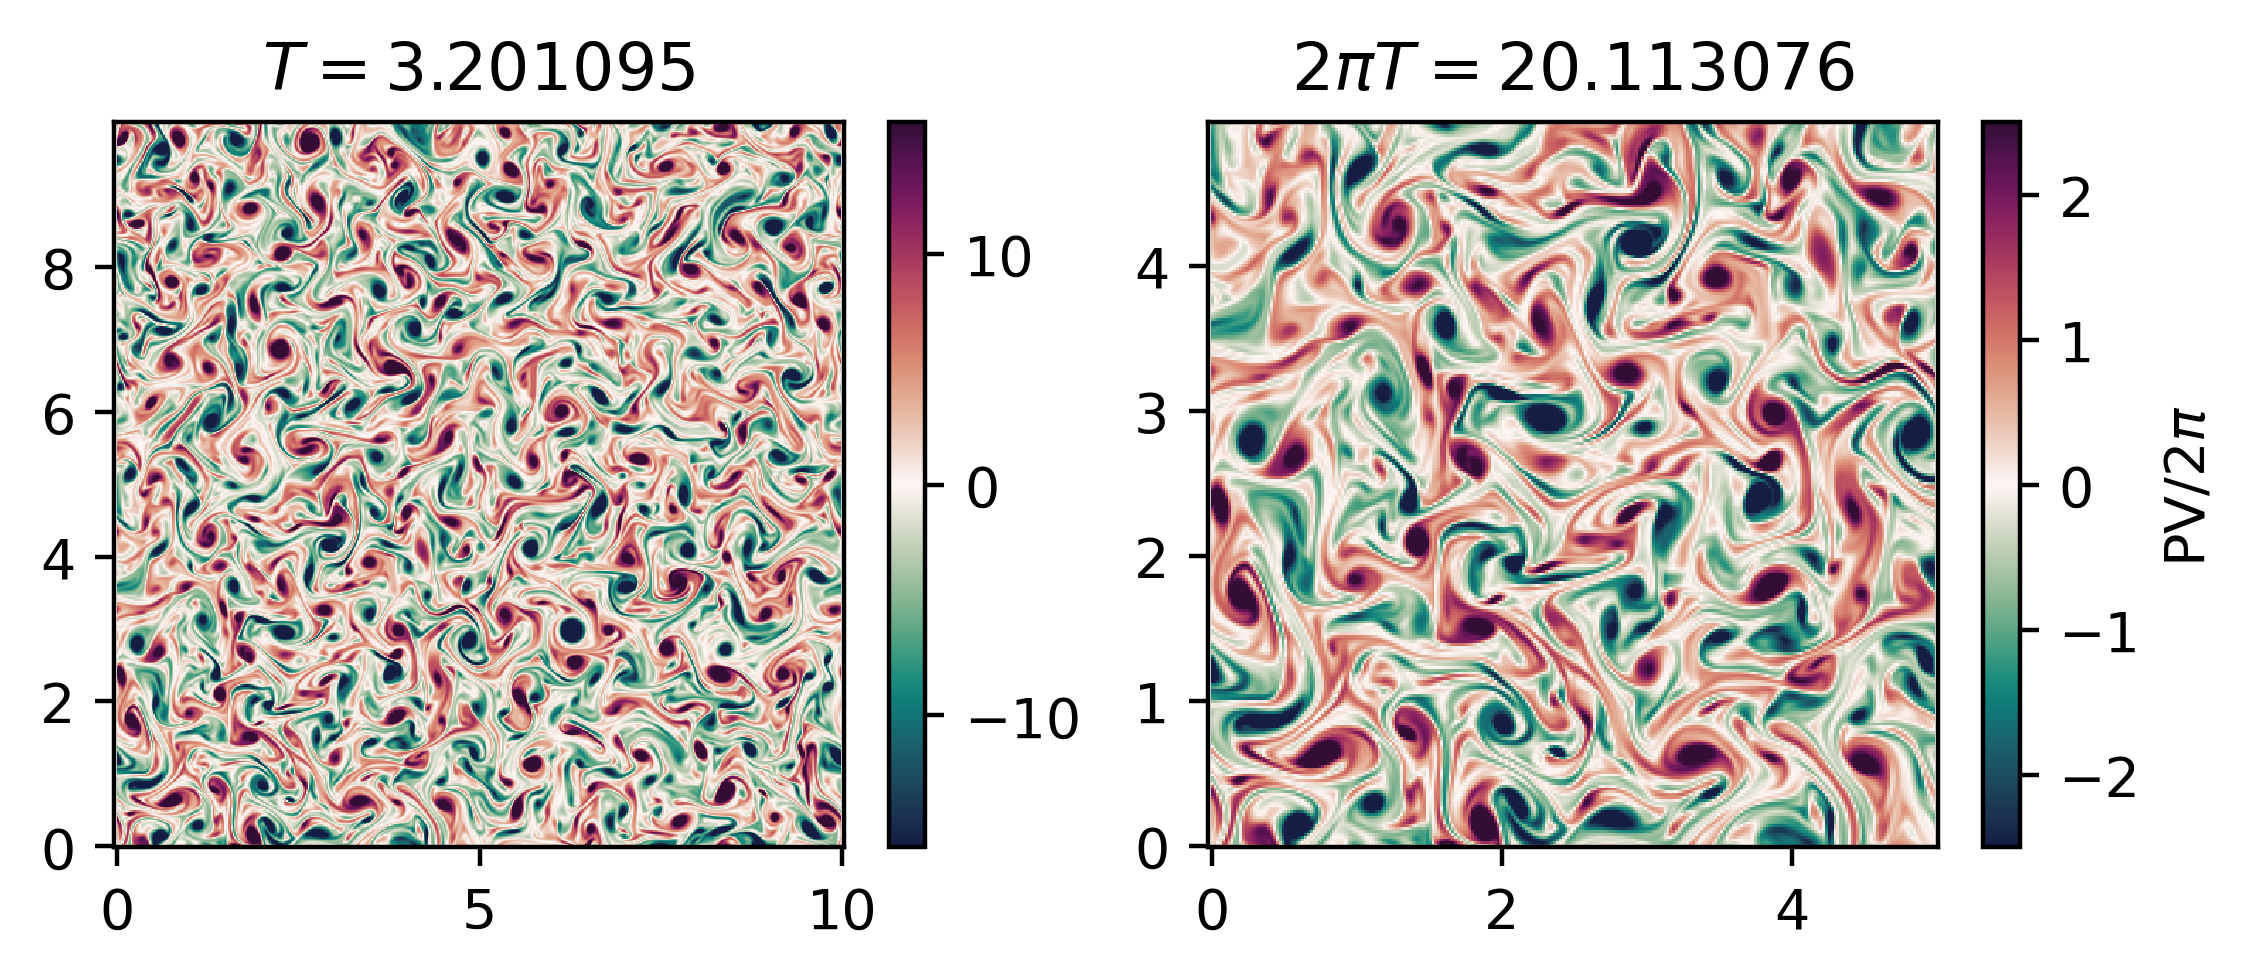
\includegraphics{PVbalanced}
    \caption{Left: the entire PV field. Right: a zoomed in picture of $(1/2)^2$ of the domain, with time and PV scaled so that to match the numbers of \cite{RochaEtAl_18}.}
    \label{fig:PVbalanced}
\end{figure}

\subsection{QG-NIW Simulation}
We simulate the QG-NIW model by adding in a wave field of
\begin{align}
    \phi = \frac{1}{\sqrt{2}}(1+i)
\end{align}
on top of the above PV field. Figure \ref{fig:QGNIW_t1} shows the result. Compare this with Figure 5 of \cite{RochaEtAl_18}, the balanced field looks similar, the action density is weaker (has less variance). We are running a $512^2$ simulation instead of $1024^2$, but this should not create that much of a difference. 
\begin{figure}[h]
    \centering
    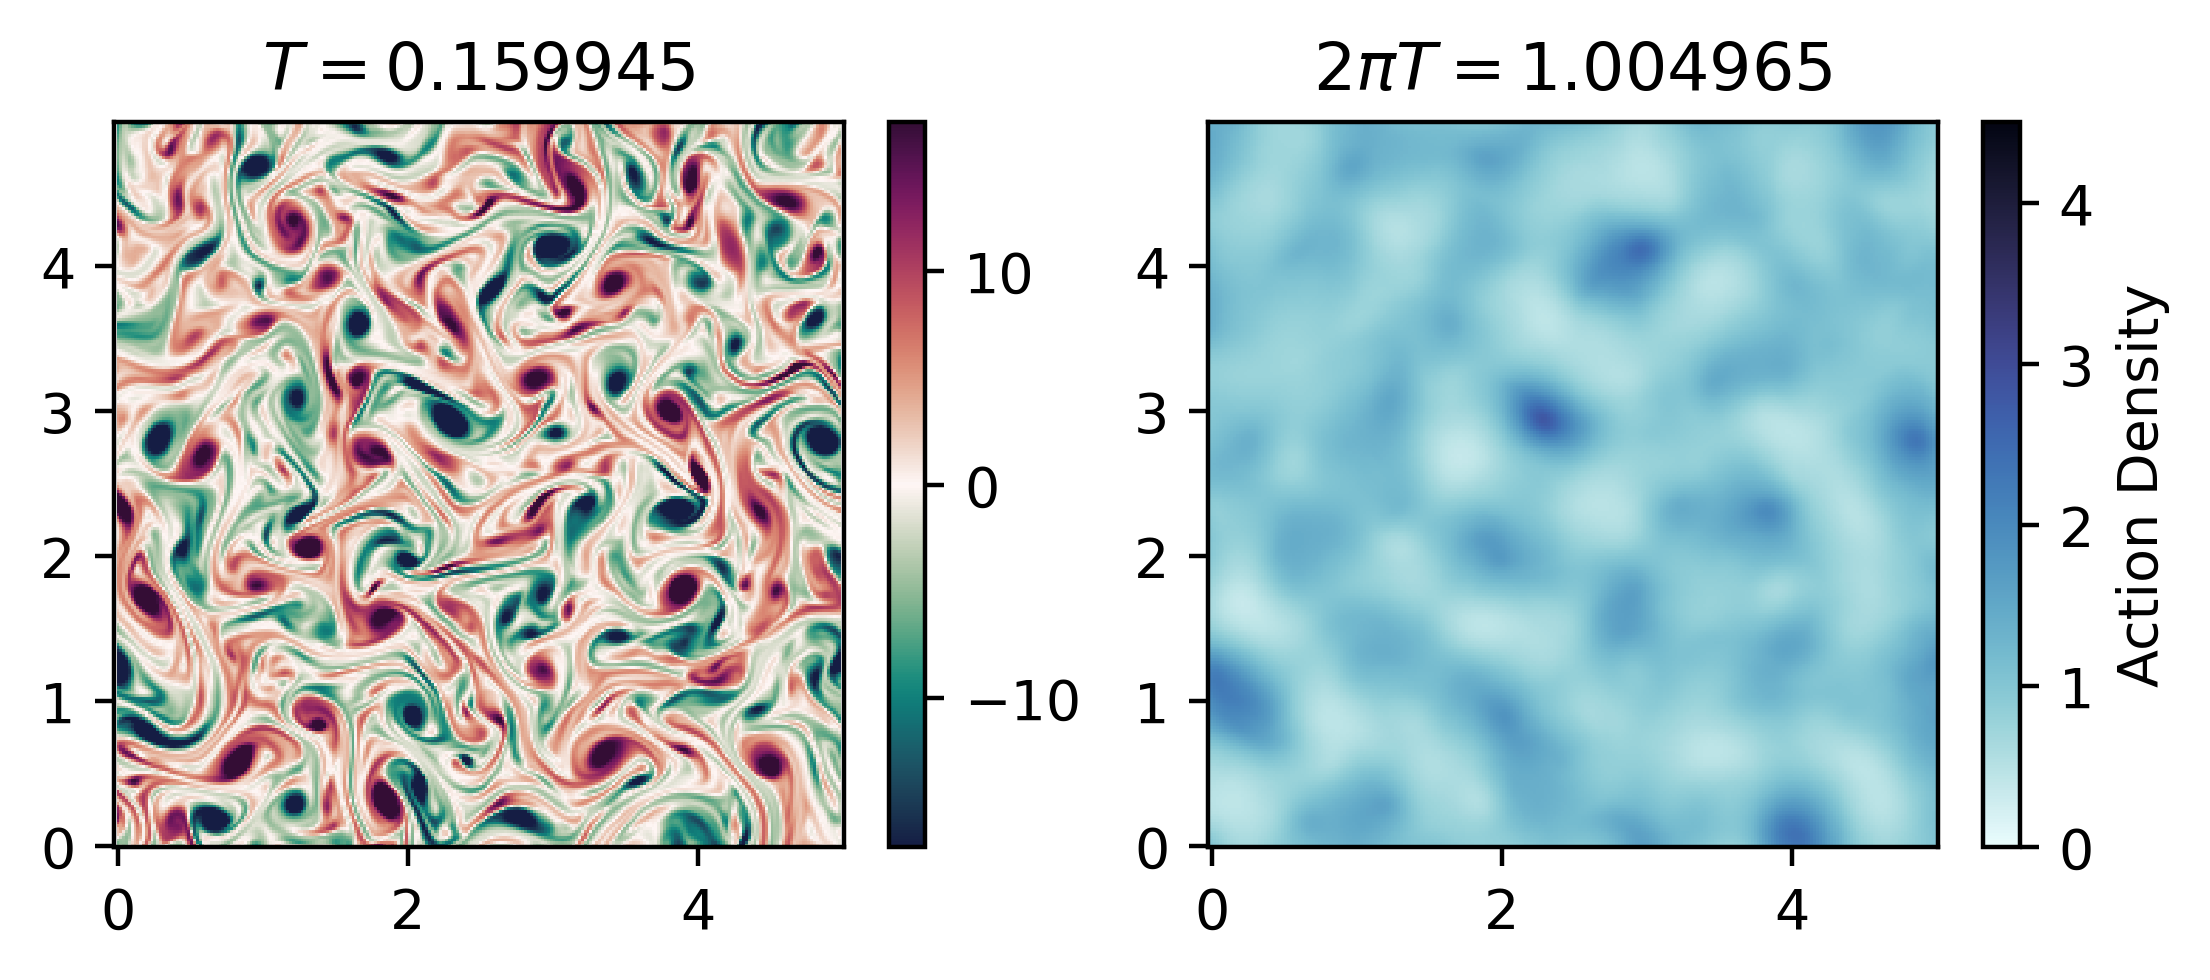
\includegraphics{QGNIW_t1}
    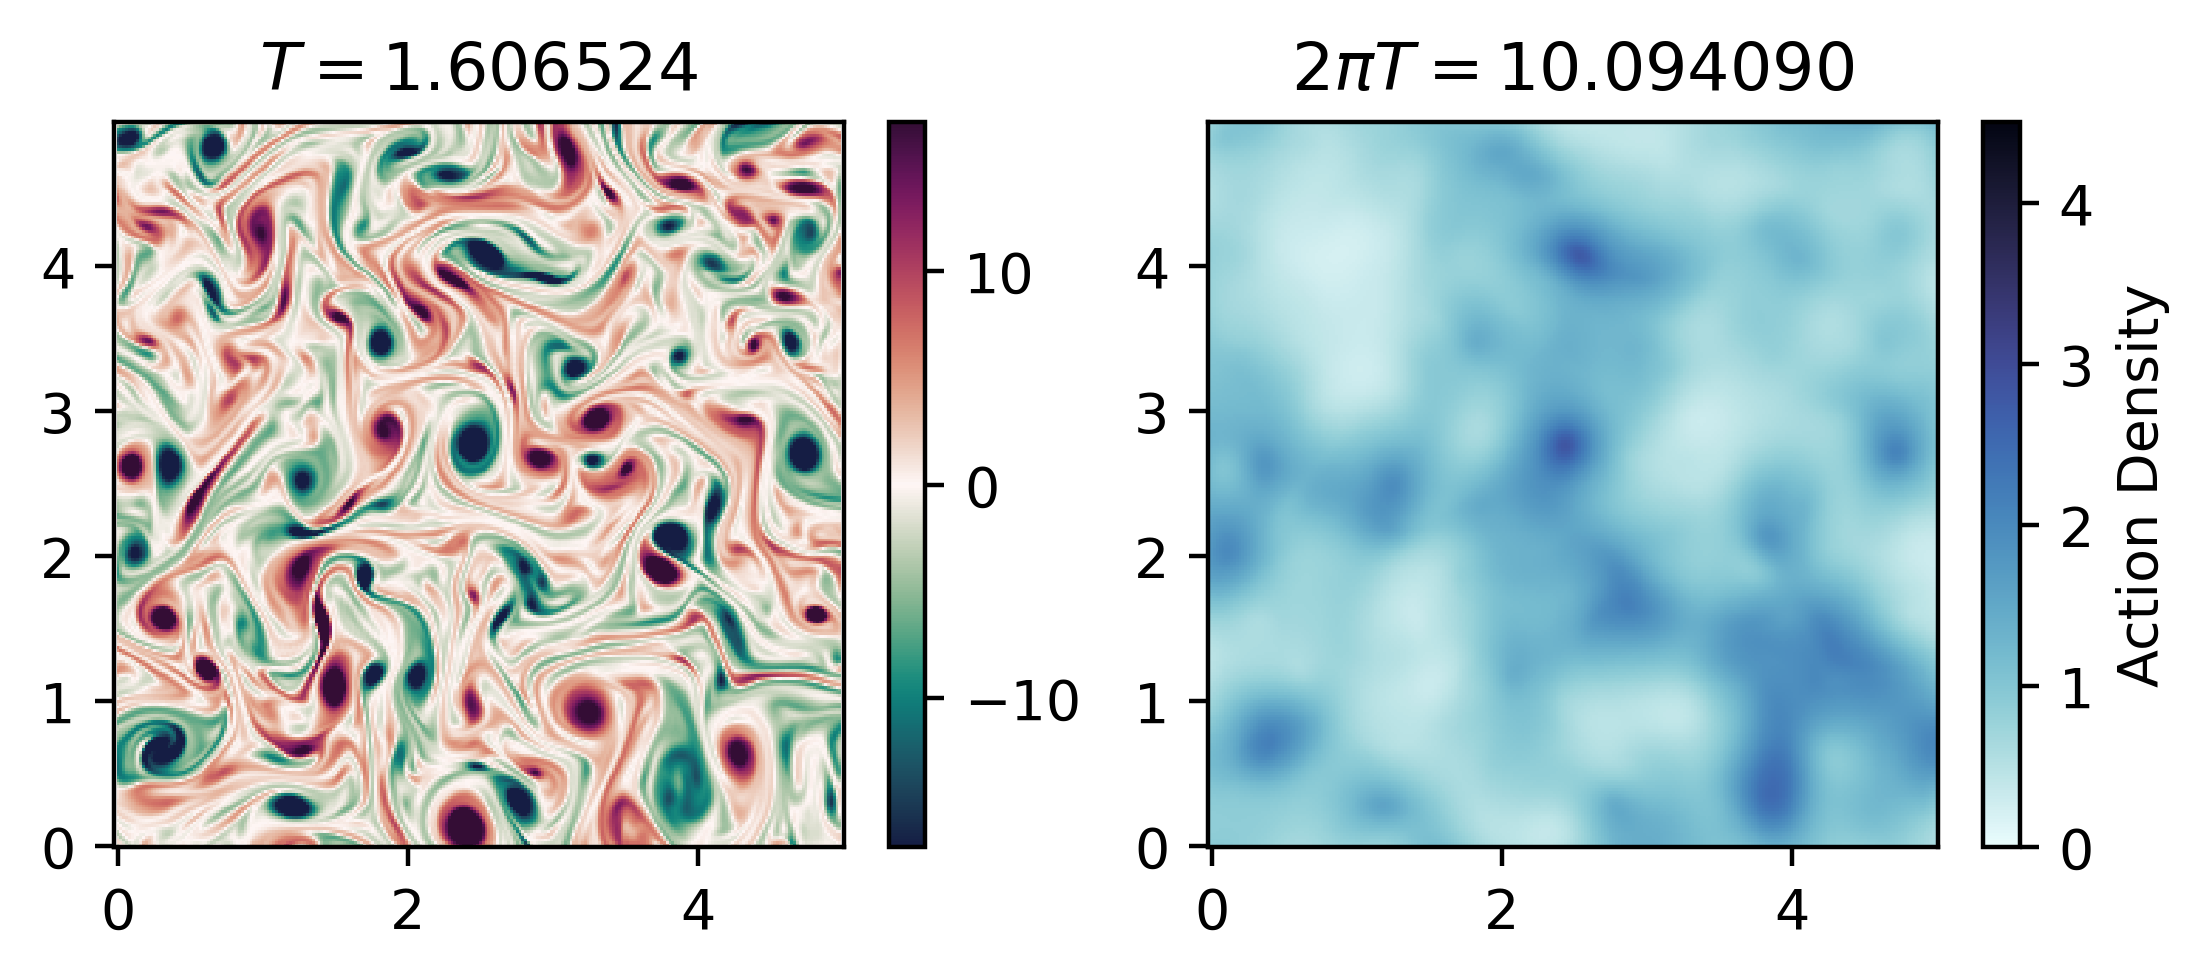
\includegraphics{QGNIW_t10}
    \caption{}
    \label{fig:QGNIW_t1}
\end{figure}

\section{Some comments}
\subsection{The IMEX time-stepper and YBJ\textsuperscript{+} equation}
We use the 3rd-order 4-stage DIRK+ERK scheme (\texttt{RK443}) for time integration \parencite[Sec 2.8]{AscherEtAl_97}. It enjoys the property that the stability region of RK4 includes a portion of the imaginary axis. This is crucial for the stable evolution of the $\phi$ equation. It is also an implicit-explicit (IMEX) method that treat the stiff linear terms implicitly. This include the $\nabla^2\phi$ term in \eqref{eq:QGNIW_eq3}. Therefore we can simulate the original QG-NIW system as written in \cite{XieVanneste_15} and \cite{RochaEtAl_18} at high resolution with reasonable timestep size. \cite{AsselinYoung_19} has modified the $\nabla^2\phi$ term in their YBJ\textsuperscript{+} equation so that the wave frequency asymptotes to twice the inertial frequency $2f$, instead of growing as $k^2$. They cite this allows explicit time-stepping of their equations. While this is true, we think this improvement is inconsequential since all turbulence simulation needs small scale dissipation, which is as stiff or stiffer than $k^2$. We have to treat stiff linear terms implicitly anyway. 

The YBJ\textsuperscript{+} equation in \cite{AsselinYoung_19} has other benefits of course, and we would like to simulate it in Dedalus. However, we need to be able to define an unusual linear operator, $\mcal{P}$ in \cite[(3.2)]{Xie_20}, in Dedalus. It is currently unclear to us on how to do this. For more see the comments in \ref{sec:ded_want_linop}.

\subsection{Another implementation in v2}
A Dedalus solver for QG-NIW also exists using Dedalus version 2 \parencite{Conn_2023}. The current implementation uses the more recent version 3, which is being actively updated. For example, Dedalus only recently (June 25, 2023)\footnote{\url{https://github.com/DedalusProject/dedalus/commit/d3843a7394e06c05bf56ba2710723e42ba19ef39}\;} allowed restart with partial data in v3 (the \verb|allow_missing| flag in \verb|solver.load_state|). Additionally, our version adaptively changes the timestep, therefore is more efficient. 


\chapter{The Quasi-Geostrophic (QG) model}
\cftchapterprecis{Ryan Sh\`iji\'e D\`u}
\graphicspath{{QG/code/}}
\renewcommand{\Bu}{\text{Bu}}
\renewcommand{\Ub}{\text{Bu}^{-1}}

\section{Barotropic QG model}
We have
\begin{align}
    &\frac{\DD}{\DD t} q+\{\xi^{-2}\}\beta v = 0,\\
    &q = \nabla^2\psi - \{\Bu^{-1}\} k_d^2\psi,\\
    &u = -\frac{\pe\psi}{\pe y}, v = \frac{\pe\psi}{\pe x}.
\end{align}
where the 
\begin{align}
    \xi^{-2} = \frac{\beta L^2}{U} \qdt{,} \text{Bu} = \frac{gH}{f_0^2L^2} = \frac{L_{d}^2}{L^2}
\end{align}

\subsection{Nonlinear freely decaying simulation}
This is an easy modification of the barotropic vorticity code.

\subsection{Rossby wave}
We simulate finite deformation radius Rossby waves in a circle gyre. There is no mean flow $U$ in this example. We use the linear barotropic QG model. That is, we use \parencite[(6.64)]{Vallis_17}:
\begin{align}
    &\frac{\pe}{\pe t} q+\{\xi^{-2}\}\beta v = 0,\\
    &q = \nabla^2\psi - \{\Bu^{-1}\} k_d^2\psi,\\
    &u = -\frac{\pe\psi}{\pe y}, v = \frac{\pe\psi}{\pe x}.
\end{align}
Standard derivation gives the dispersion relation for this Rossby wave \parencite[(RW.3)]{Vallis_17}:
\begin{align}
    \omega = \frac{-\{\xi^{-2}\}\beta k}{k^2+\ell^2+\{\Bu^{-1}\}k_d^2}
\end{align}
We then have the phase velocity in the $x$-direction is
\begin{align}
    c_p^x = \frac{\omega\cdot k}{(k^2+\ell^2)} = \frac{-\{\xi^{-2}\}\beta k^2}{(k^2+\ell^2+\{\Bu^{-1}\}k_d^2)(k^2+\ell^2)}<0.
\end{align}
The group velocity is \parencite[(RW.4)]{Vallis_17}
\begin{align}
    c_g^x = \frac{\pe\omega}{\pe k} = \frac{\{\xi^{-2}\}\beta(k^2-\ell^2-\{\Bu^{-1}\}k_d^2)}{(k^2+\ell^2+\{\Bu^{-1}\}k_d^2)}.
\end{align}
We see that the phase velocity of the Rossby wave is always westward ($\beta>0$ always), while the group velocity's direction depends on the spatial scale of the wave.

We simulate Rossby waves with $\Bu=1$ an $\xi^{-2}=1$ to focus on the effects of wave size. First, we make a wave package with $k=0.7$ and $\ell=0$. We plot the wave after some time in Figure \ref{fig:Rossby_k0d7_tt20d11}. It is clear that the group velocity is westward because the package has moved west. To see that the phase velocity is westward, please watch the \href{https://vimeo.com/936333986}{video}. 

\begin{figure}
    \centering
    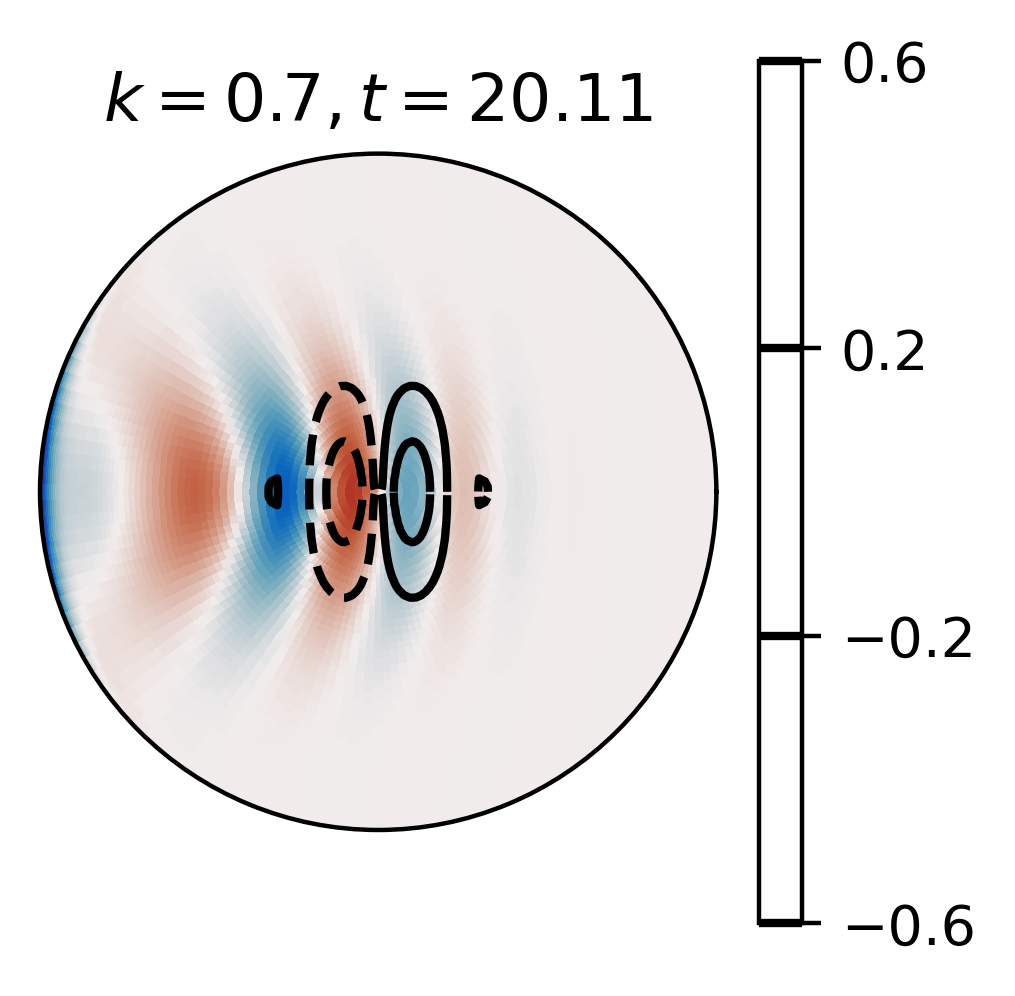
\includegraphics{Rossby_plots/Rossby_k0d7_tt20d11}
    \caption{}
    \label{fig:Rossby_k0d7_tt20d11}
\end{figure}

\href{https://vimeo.com/936333886}{video}. 


% \section{The full model nondimensionalized}
% We start with the 2 layer QG model with mean flow, $\beta$, and topography \parencite[(5.85-86)]{Vallis_17} (in the notation of \cite{Vallis_96a}):
% \begin{align}
%     &\frac{\pe q_1}{\pe t}+J(\psi_1,q_1)+U_1\frac{\pe q_1}{\pe x}+\left(\{\xi_1^{-2}\}\beta+\{\Bu_1^{-1}\}\frac{f_0^2(U_1-\{U_r\}U_2)}{g'H_1}\right)\frac{\pe\psi_1}{\pe x} = 0;\label{eq:2lay_eq1}\\
%     \{A\}&\frac{\pe q_2}{\pe t}+J(\psi_2,q_2)+U_2\frac{\pe q_2}{\pe x}+\left(\{\xi_2^{-2}\}\beta+\{\Bu_2^{-1}\}\frac{f_0^2(U_2-\{U_r^{-1}\}U_1)}{g'H_2}\right)\frac{\pe\psi_2}{\pe x} = 0.\label{eq:2lay_eq2}
% \end{align}
% where
% \begin{align}
%     q_1 &= \nabla^2\psi_1 + \{\Bu_1^{-1}\}\frac{f_0^2}{g'H_1}(\{U_r\}\psi_2-\psi_1);\label{eq:2lay_pv1}\\
%     q_2 &= \nabla^2\psi_2 + \{\Bu_2^{-1}\}\frac{f_0^2}{g'H_2}(\{U_r^{-1}\}\psi_1-\psi_2)+\left\{\frac{\alpha}{\text{Ro}_2}\right\}\frac{f_0}{H_2}\eta.\label{eq:2lay_pv2}
% \end{align}
% We have nondimensionalized time to be the advective timescale of the first layer:
% \begin{align}
%     T = \frac{L_1}{U_1}.
% \end{align}
% Then we nondimensionalized \eqref{eq:2lay_eq1} and \eqref{eq:2lay_pv1} with length $L_1$ and \eqref{eq:2lay_eq2} and \eqref{eq:2lay_pv2} with length $L_2$. We have introduced the nondimensional number $\xi$ which is the ratio between the Rhine scale and the lengthscale of each layer \parencite{HeldLarichev_96}
% \begin{align}
%     \xi_i^{-2} = \frac{\beta L_i^2}{|U_i|}
% \end{align}
% and $\alpha$ which is the ratio of the typical topographic height versus the second layer's height
% \begin{align}
%     \alpha = \frac{\eta}{H_2}.
% \end{align}
% If the height and mean flow of the two layers are not equal, we have two parameters for their ratio
% \begin{align}
%     U_r = \frac{|U_2|}{|U_1|}, \qdt{and} A = \frac{|U_1|L_2}{|U_2|L_1}
% \end{align}
% We also have the more familiar quantities
% \begin{align}
%     L_{i,d} = \frac{\sqrt{g'H_i}}{f_0} \qdt{,} \text{Ro}_2 = \frac{|U_2|}{f_0L_2} \qdt{and} \text{Bu}_i = \frac{L_{i,d}^2}{L_i^2}.
% \end{align}

\section{The 2-layer QG model under Phillips baroclinic instability}
\subsection{The nondimensional equations}
The 2-layer model simplifies drastically when we make the upper/lower layer symmetry assumption \parencite{LarichevHeld_95}. We take $H_1=H_2 = H/2$ and $U_1=-U_2=U$. Then the equation becomes
\begin{align}
    &\frac{\pe q_1}{\pe t}+J(\psi_1,q_1)+U\frac{\pe q_1}{\pe x}+\left(\{\xi^{-2}\}\beta+\{8\Bu^{-1}\}\frac{4f_0^2U}{g'H}\right)\frac{\pe\psi_1}{\pe x} = 0,\label{eq:2lay_sym_eq1}\\
    &\frac{\pe q_2}{\pe t}+J(\psi_2,q_2)-U\frac{\pe q_2}{\pe x}+\left(\{\xi^{-2}\}\beta-\{8\Bu^{-1}\}\frac{4f_0^2U}{g'H}\right)\frac{\pe\psi_2}{\pe x} = 0;\label{eq:2lay_sym_eq2}
\end{align}
where
\begin{align}
    q_1 &= \nabla^2\psi_1 + \{4\Bu^{-1}\}\frac{2f_0^2}{g'H}(\psi_2-\psi_1),\label{eq:2lay_sym_pv1}\\
    q_2 &= \nabla^2\psi_2 + \{4\Bu^{-1}\}\frac{2f_0^2}{g'H}(\psi_1-\psi_2)+\left\{\frac{\alpha}{\text{Ro}}\right\}\frac{2f_0}{H}\eta.\label{eq:2lay_sym_pv2}
\end{align}
We have 
\begin{align}
    \xi^{-2} = \frac{\beta L^2}{U} \qdt{,} \text{Bu} = \frac{2g'H}{f_0^2L^2} = \frac{L_{d}^2}{L^2} \qdt{and} \alpha = \frac{2\eta}{H}.
\end{align}
Note that this implies (cf. \cite[(9.103)]{Vallis_17})
\begin{align}
    L_d = \frac{2\sqrt{g'H/2}}{f_0} \qdt{with} k_d^2 = \frac{4f_0^2}{g'H} = \frac{8}{L_d^2}.
\end{align}
This is an ok definition when we connect to the continuously stratified case by using (cf. \cite[(5.138)]{Vallis_17})
\begin{align}
    L_d = \frac{NH}{f} \qdt{with} N^2 = \frac{g'}{H/2}.
\end{align}
$\xi$ and $\Bu$ are not independent since their only freedom is in picking $L$. In our simulation, we pick $L=L_d$ such that $\text{Bu}=1$. 
We further simplify by setting flat topography ($\alpha=0$). The only free parameter is $\xi$
\begin{align}
    \xi^{-2}= \frac{\beta L^2}{U} = \frac{\beta L_d^2}{U}
\end{align}
It is the two-layer version of the `Charney–Green number’. 

Finally, we simulate using a $|k|^8$ hyper-diffusivity on $q_i$ for small scale dissipation and an Ekman damping only in the bottom layer for damping the inverse cascade.

\subsection{Linear stability analysis}
We take only the linear terms of the above model, and dispense of all unnecessary parameters:
\begin{align}
    &\frac{\pe q_1}{\pe t}+\frac{\pe q_1}{\pe x}+\left(\xi^{-2}+8\Bu^{-1}\right)\frac{\pe\psi_1}{\pe x} = 0,\label{eq:2lay_sym_eq1_lin}\\
    &\frac{\pe q_2}{\pe t}-\frac{\pe q_2}{\pe x}+\left(\xi^{-2}-8\Bu^{-1}\right)\frac{\pe\psi_2}{\pe x} = 0;\label{eq:2lay_sym_eq2_lin}
\end{align}
where
\begin{align}
    q_1 &= \nabla^2\psi_1 + 4\Bu^{-1}(\psi_2-\psi_1),\label{eq:2lay_sym_pv1_lin}\\
    q_2 &= \nabla^2\psi_2 + 4\Bu^{-1}(\psi_1-\psi_2).\label{eq:2lay_sym_pv2_lin}
\end{align}

This system if isomorphic to \cite[(9.107)]{Vallis_17}. Therefore we can copy down the answer:
\begin{align}
    c &= -\frac{\xi^{-2}}{K^2+8\Bu^{-1}}\left\{ 1+\frac{8\Bu^{-1}}{2K^2}\pm\frac{8\Bu^{-1}}{2K^2}\left[1+4\frac{K^4(K^4-8^2\Bu^{-2})}{8^2\xi^{-4}\Bu^{-2}}\right]^{1/2} \right\}.
\end{align}
We have recovered \cite[(9.114)]{Vallis_17} with $\hat{k}_d^2 = 8$ and (cf. \cite[(9.115)]{Vallis_17})
\begin{align}
    \xi^{-2} = \hat{k}_\beta^2 = \frac{\beta L_d^2}{U}.
\end{align}

Now we can use the eigenvalue-problem module of Dedalus is solve the same problem numerically. Figure \ref{fig:2Lay_linstab} shows the growth rate. This is a reproduction of \cite[Fig. 9.14]{Vallis_17}.
\begin{figure}
    \centering
    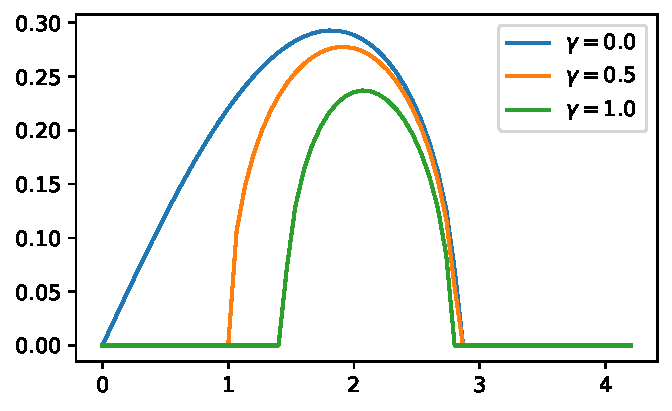
\includegraphics{plot_snap/figs/2Lay_linstab}
    \caption{}
    \label{fig:2Lay_linstab}
\end{figure}


\subsection{Simulation of jets formation}
We pick $\xi = 0.4$ for a large $\zeta$ effect while still having a baroclinically unstable background. At early times, baroclinic instability appears with its distinct pattern. In Figure \ref{fig:2Layjets_q1_t6d50} we also plot a sin wave with $2.26$ wavenumber, the fastest growing mode for $\xi = 0.4$. We see that the instability pattern matches the theory. At later times, the flow develops into jets. Figure \ref{fig:2Layjets_q1_t150d00} shows clear PV staircases with homogenized regions in between. Figure \ref{fig:2Layjets_q1zonalmean_t150d00} plots the zonally averaged perturbation PV $q_1$ against a sin wave of wavenumber $1/2\xi$. We see that matches well the distance between jets. Note that
\begin{align}
    \frac{1}{2\xi} = \frac{1}{2}\hat{k}_\beta = \sqrt{\gamma}
\end{align}
where $\gamma$ is defined in \cite[(9.115)]{Vallis_17}. 

\begin{figure}
    \centering
    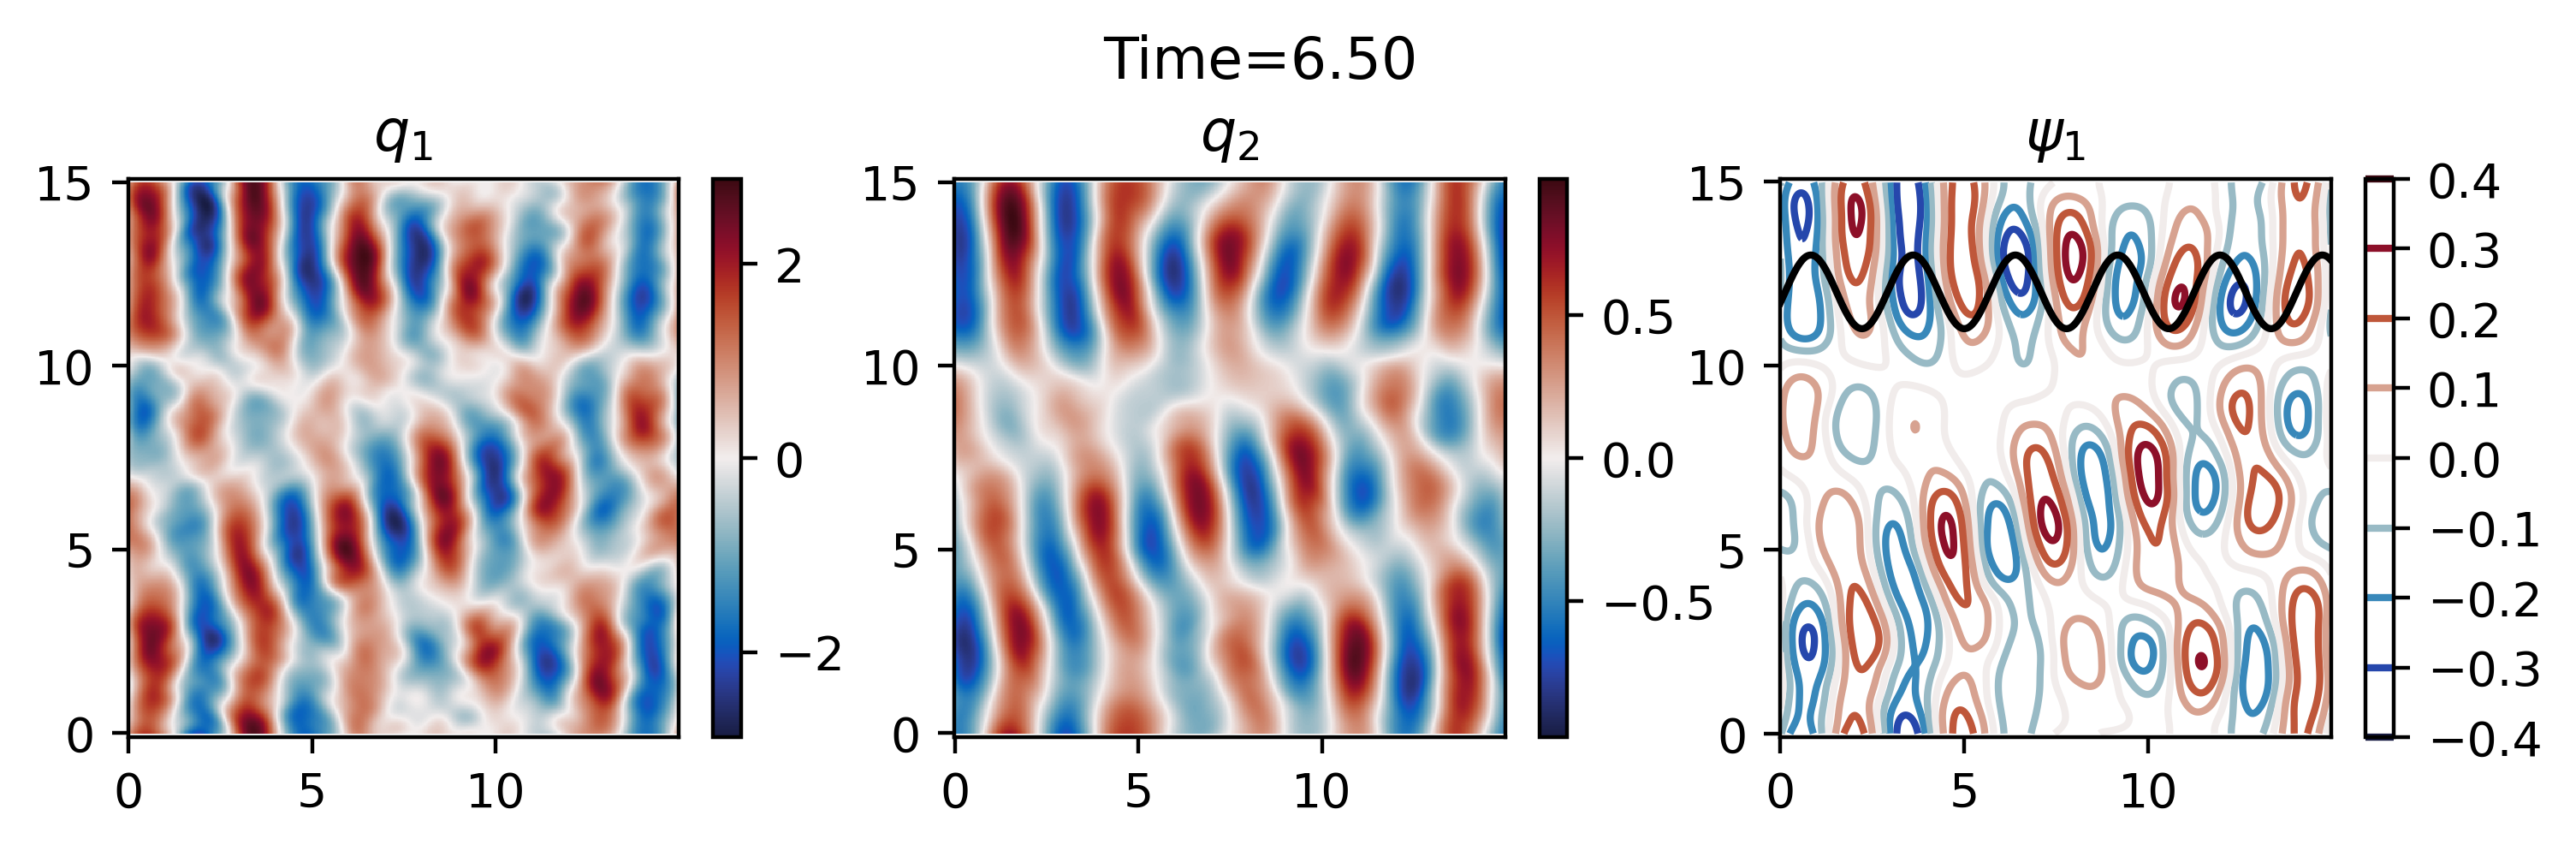
\includegraphics[width=\textwidth]{plot_snap/figs/2Layjets_q1_t6d50}
    \caption{}
    \label{fig:2Layjets_q1_t6d50}
\end{figure}


\begin{figure}
    \centering
    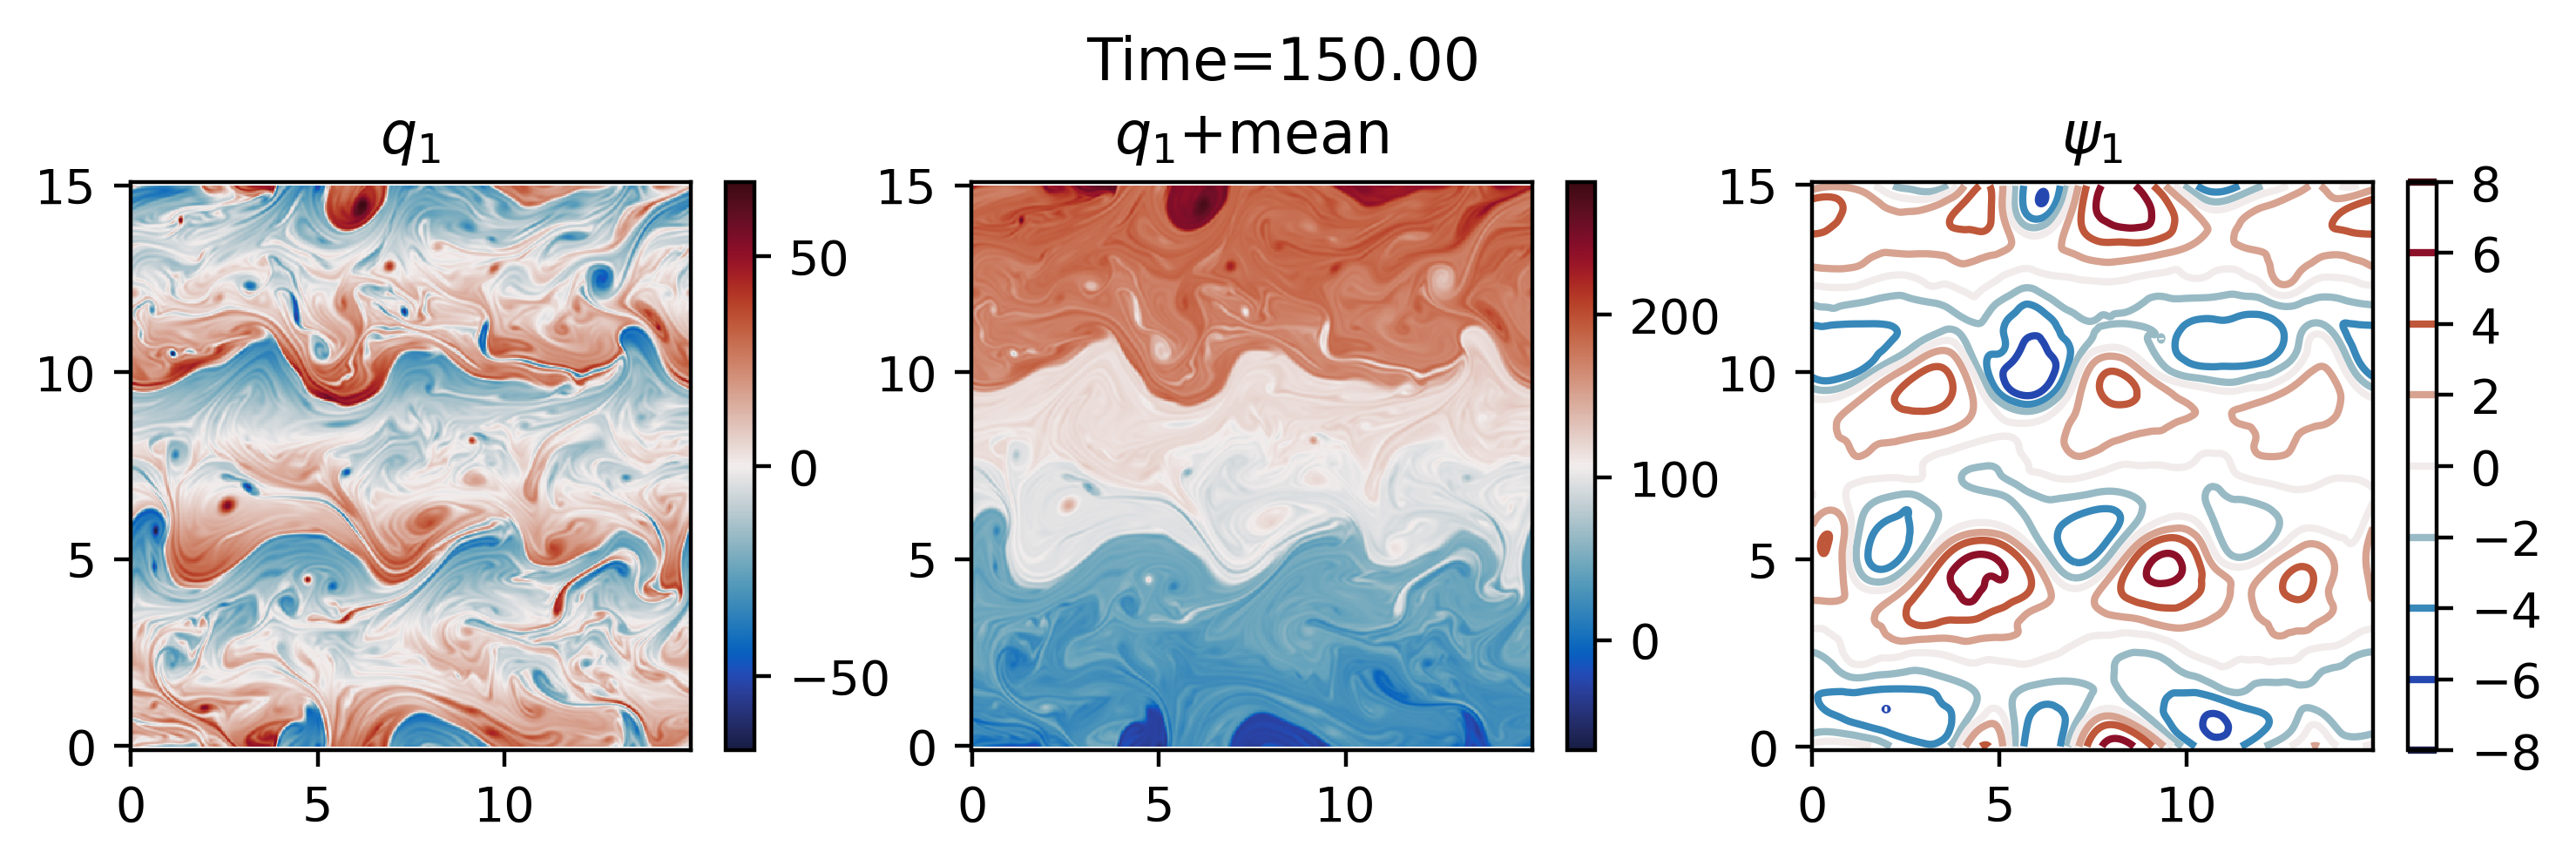
\includegraphics[width=\textwidth]{plot_snap/figs/2Layjets_q1_t150d00}
    \caption{}
    \label{fig:2Layjets_q1_t150d00}
\end{figure}

\begin{figure}
    \centering
    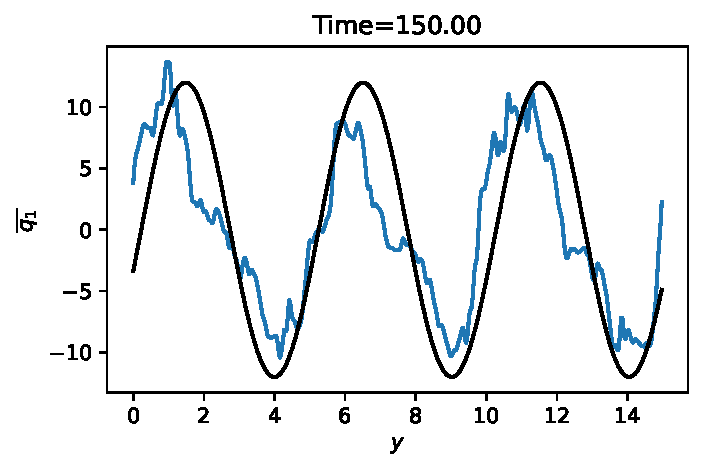
\includegraphics{2Layjets_q1zonalmean_t150d00}
    \caption{}
    \label{fig:2Layjets_q1zonalmean_t150d00}
\end{figure}

\subsection{2 layer turbulence}
We instead pick $\xi=1.5$ on a larger domain for a simulation with small $\beta$ effect. Figure \ref{fig:2Lay_qbrbc_t150d00} shows the barotropic and baroclinic PV. These are visually similar to \cite[Fig. 3]{LarichevHeld_95}. We also plot the $q_1$ enstrophy spectrum in Figure \ref{fig:2Lay_q1spec_t150d00}. The spectrum has a slope of $-1$, matching the theoretical expectation.

\begin{figure}
    \centering
    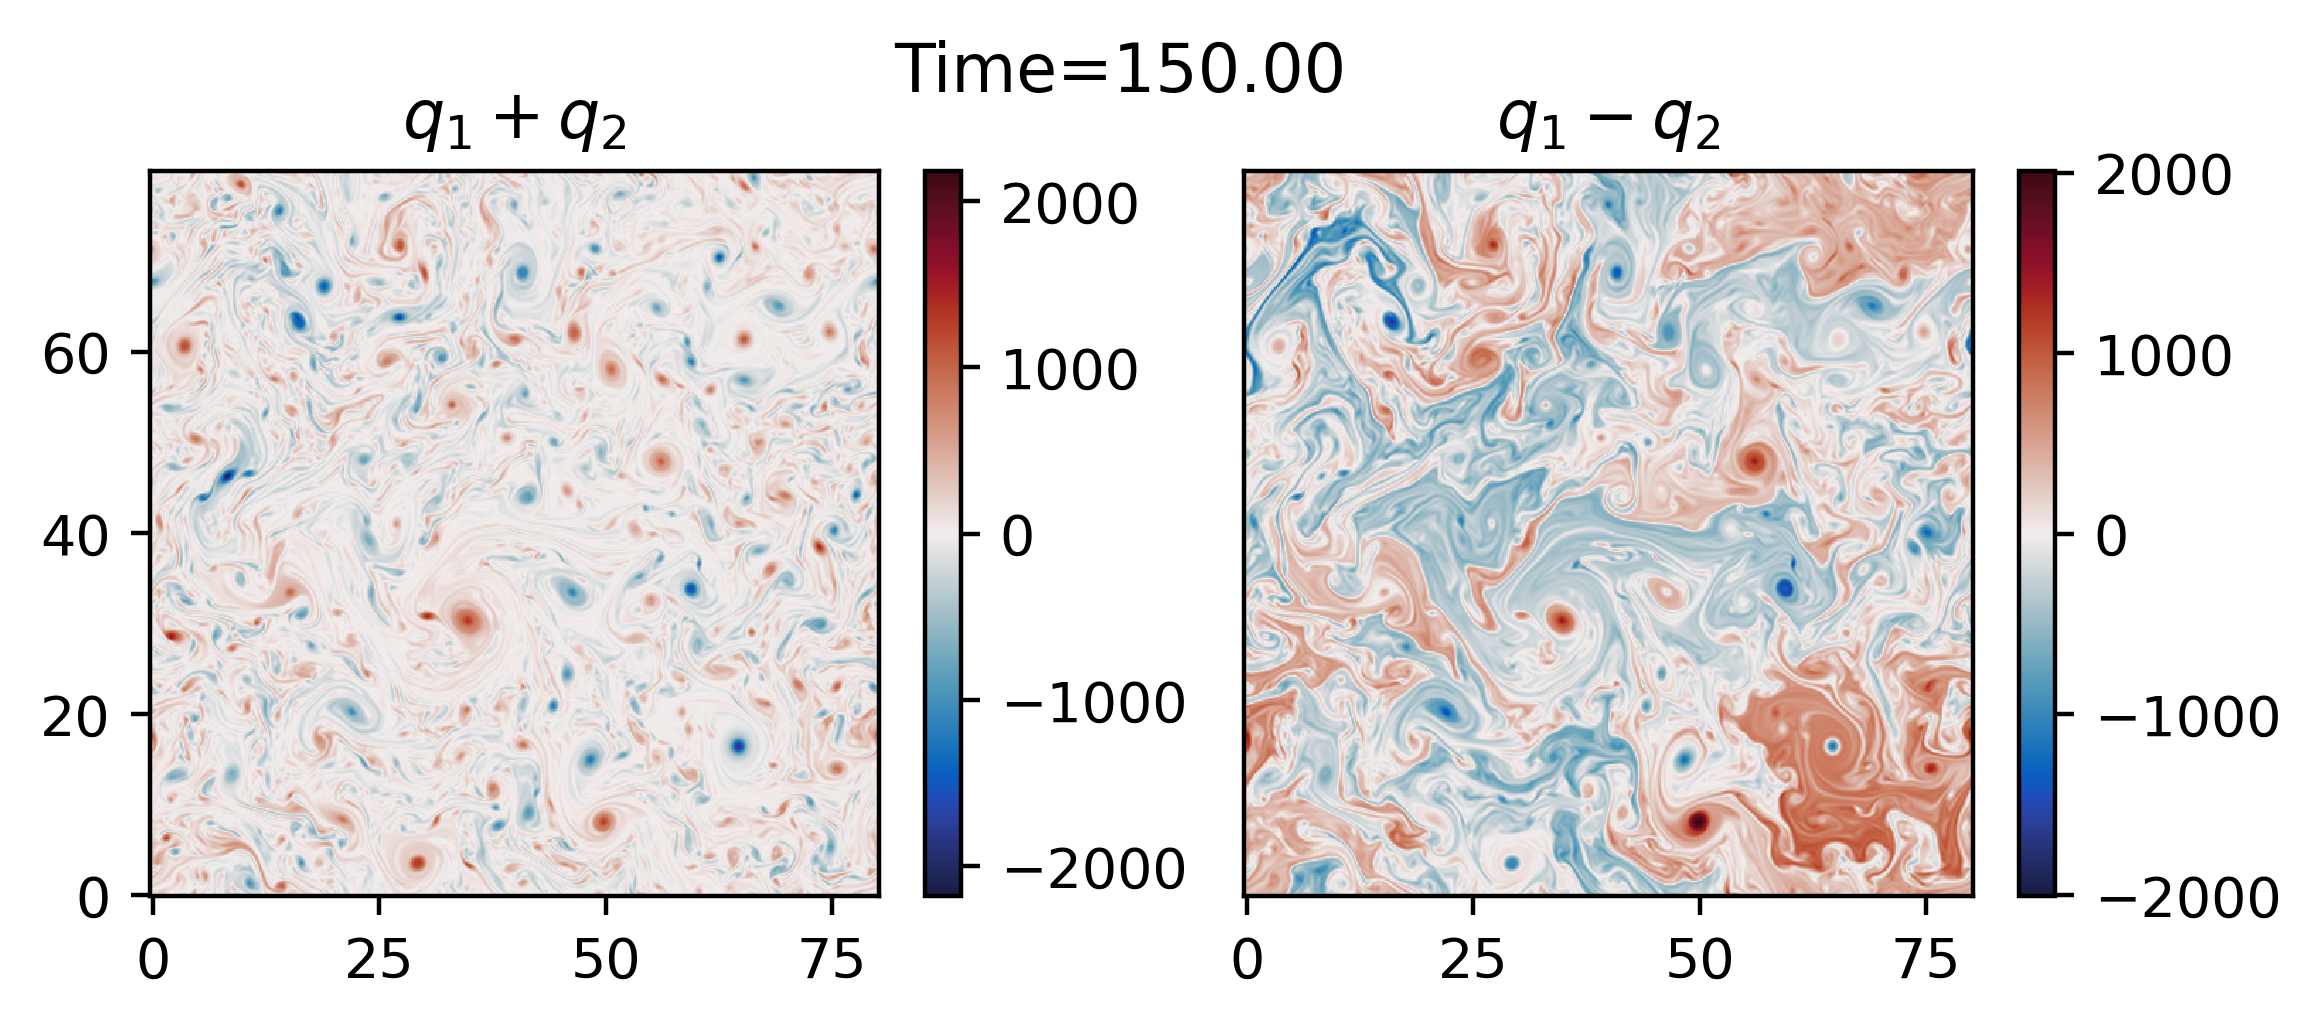
\includegraphics{plot_snap/figs/2Lay_qbrbc_t150d00}
    \caption{}
    \label{fig:2Lay_qbrbc_t150d00}
\end{figure}

\begin{figure}
    \centering
    
\includegraphics{plot_snap/figs/2Lay_q1spec_t150d00}
    \caption{}
    \label{fig:2Lay_q1spec_t150d00}
\end{figure}

\chapter{Baroclinic mode}
\cftchapterprecis{Ryan Sh\`iji\'e D\`u}
\graphicspath{{Baroclinic_mode/code/figs/}}

We solve the baroclinic mode for arbitrary stratification profiles. That is, we solve the Sturm–Liouville problem:
\begin{align}
&\frac{\mathrm{d}}{\mathrm{d}z}\left( \frac{f^2}{N^2}\frac{\mathrm{d}\psi}{\mathrm{d}z} \right) = -\lambda^2\psi\\
\text{with}\qquad &\frac{\mathrm{d}\psi}{\mathrm{d}z}(z=0)=\frac{\mathrm{d}\psi}{\mathrm{d}z}(z=-H)=0
\end{align}
where $N^2$ is a function of $z$.

We pose the problem on $H\in[-1,0]$ with $f^2/N^2(z)=e^{z}$. Realistic physical values only change the eigenvalues by a constant. We use the eigenvalue problem module of Dedalus. The eigenvalues and eigenvectors (the baroclinic mode) are shown in Figure \ref{fig:expo_bc_mode}.

\begin{figure}
    \centering
    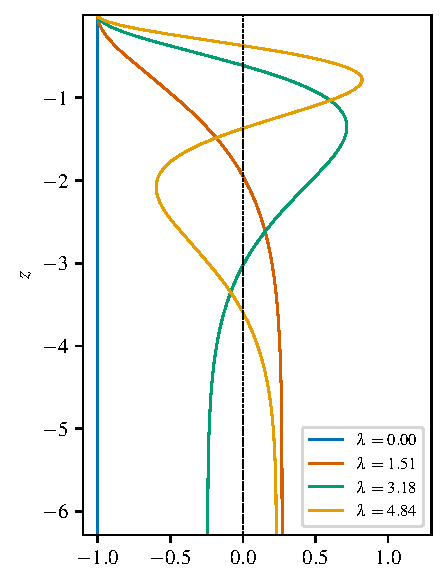
\includegraphics{expo_bc_mode}
    \caption{}
    \label{fig:expo_bc_mode}
\end{figure}

There are many definitions of orthogonal vertical mode for the ocean. For some examples, see \cite{SmithVanneste_13,LaCasce_17,YassinGriffies_22}. All these problems can be solved by Dedalus, with more or less modification of the above code. One could also input realistic stratification profiles from data, interpolating them onto a Chebyshev grid of sufficient resolution. In particular, this code reproduces the functionality of \url{https://github.com/rabernat/oceanmodes}. 

\chapter{Linear instability of 3DQG}
\cftchapterprecis{Ryan Sh\`iji\'e D\`u}
\graphicspath{{3DQG_Linstab/code/figs/}}

In this chapter, we give examples of how to use the eigenproblem model of Dedalus. In particular, we show how to extract eigenvectors when the problem is complex. This is not shown in the examples on the official website. To do this, we solve the linear instability analysis problem of three-dimensional baroclinic instability in the quasi-geostrophic (QG) model.

\section{The 3DQG model under baroclinically unstable mean states}
We have the 3D QG model in the $\beta$-plane under the mean zonal velocity $U(z)$. We have the surface meridional buoyancy gradient $B_y(z=-H, 0)$ from thermal wind balance. This also implies a mean meridional PV gradient
\begin{align}
    Q_y = \{\xi^{-2}\}\beta-\nabla^2 U-\{\Bu^{-1}\}\frac{\de}{\de z}\left(\frac{f^2}{N^2}\frac{\de U}{\de z}\right)
\end{align}
where we ignore the $\nabla^2 U$ term with our assumption that $U$ is horizontally constant. Now we have the 3DQG system:
\begin{align}
    &\frac{\DD q}{\DD t}+Uq_x+vQ_y = 0; \\
    &\frac{\DD b}{\DD t}+Ub_x+vB_y = 0 \qdt{at} z=-H, 0; \\
    &\nabla^2\psi + \{\Bu^{-1}\}\frac{\pe}{\pe z}\left(\frac{f^2}{N^2}\frac{\pe\psi}{\pe z}\right) = q \\
    &\quad\qdt{w/} \psi_z = b/f \qdt{at} z=-H, 0; \\
    &u = -\psi_y, \quad v = \psi_x.
\end{align}
We use the nondimensional number
\begin{align}
    \xi^{-2} = \frac{f_0 L}{U} \qdt{,} \Bu = \frac{N(0)^2H^2}{f_0^2L^2} = \frac{L_{d}^2}{L^2}.
\end{align}
Finally for the linear instability analysis we form a linear system by assuming small perturbation and ignoring all quadratic in perturbation terms. We then solve the eigenproblem of the linear system.

\section{The Eady instability}
We use Dedalus to solve the classic Eady baroclinic instability problem. For the Eady problem, the PV is assumed to be zero. Therefore we only have the advection of the buoyancy on the top and bottom. We refer to \cite[\S 9.5]{Vallis_17} for more details on the set-up of the problem and the algebraic solution. Here we use Dedalus to recover their result. Figure \ref{fig:Eady_matchvallis} matches exactly \cite[Fig. 9.10]{Vallis_17}, and Figure \ref{fig:Eady_profile} matches exactly \cite[Fig. 9.12]{Vallis_17}. It is also possible to reproduce \cite[Fig. 9.11]{Vallis_17} and is left as an exercise for the reader.

\begin{figure}
    \centering
    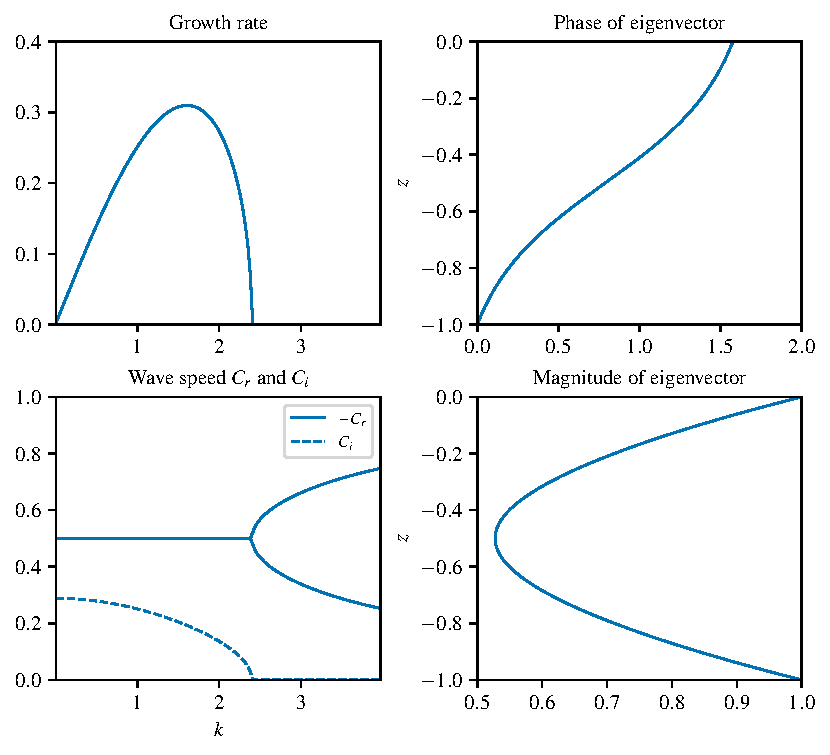
\includegraphics{Eady_matchvallis}
    \caption{Solution to the Eady problem.}
    \label{fig:Eady_matchvallis}
\end{figure}

\begin{figure}
    \centering
    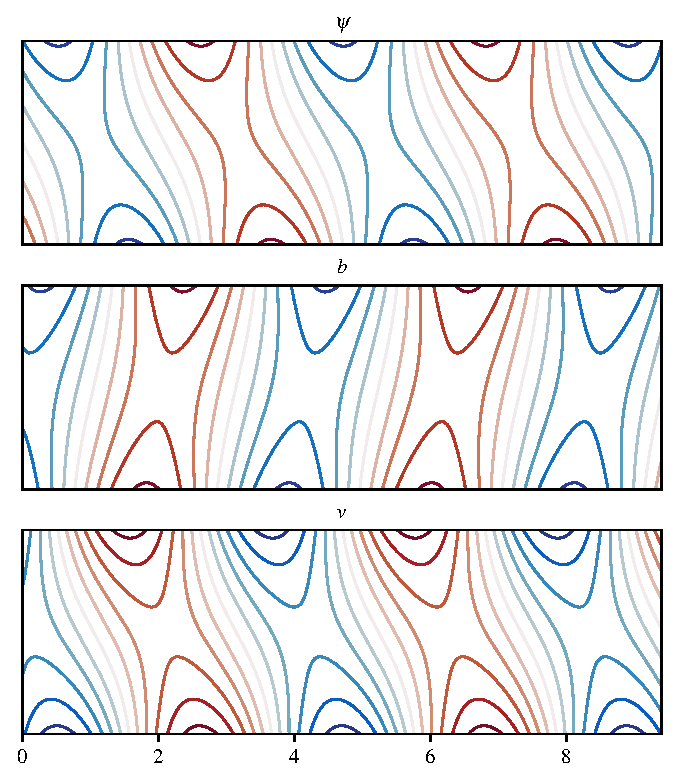
\includegraphics{Eady_profile}
    \caption{Profiles of the most unstable mode for the Eady problem.}
    \label{fig:Eady_profile}
\end{figure}

\section{The ocean Charney instability}
The Eady instability is an instability due to the interaction of two surface modes. We explore the effects of the interior PV gradient by studying the ocean Charney instability \parencite{CapetEtAl_16}. To begin, the ocean Charney instability is due to interaction between the top boundary and the interior. From the Charney–Stern–Pedlosky (CSP) condition, we know that for instability, we need $Q_y$ is the opposite sign to $U_z$ at the upper boundary \parencite[p. 351]{Vallis_17}. For the ocean, there are two ways for this to happen. For an eastward sheared top mean current $U_z>0$, we need $Q_y<0$. For this, we need the curvature of the zonal velocity to overwhelm the positive planetary PV gradient $\beta$. Now if the top mean current is westward sheared $U_z<0$, we need $Q_y>0$ which can be provided by the planetary PV gradient $\beta$. Both can happen in the ocean according to the global study of \cite{TullochEtAl_11}. We study the linear instability of both scenarios. For that, we ignore the bottom boundary by setting $b=0$ at $z=-H$.

\subsection{Idealized profiles inspired by the ocean}
For our preliminary examples to demonstrate Dedalus, we use idealized nondimensional profiles. Converting the code to take real data would be simple. 

The 3DQG system above only needs stratification $N^2(z)$ and mean velocity $U(z)$ at vertical profiles as inputs. That is the data our data will take. We will use exponential stratification
\begin{align}
    N^2(z) = N^2 e^{z/\delta} \qdt{w/} \delta=0.2.
\end{align}
For velocity we use
\begin{align}
    U(z) = (1+z-\delta)e^{z/\delta}/5.
\end{align}
We scale the velocity so that $\dsp{\frac{\pe}{\pe z}\left(\frac{f^2}{N^2}\frac{\pe\psi}{\pe z}\right)}=1$. 

\subsection{Condition for instability}
Note that in our nondimensionalization, the velocity is fixed. To compare the different cases of velocity shear, we flip the sign of $\beta$ instead by using different signs of $\xi^{-2}$. To satisfy the CSP condition, we always need 
\begin{align}
    Q_y = \{\xi^{-2}\}-1<0.
\end{align}
Therefore we need
\begin{align}
    \{\xi^{-2}\}<1.
\end{align}
Note that this means all westward mean velocity is unstable, while eastward velocity has to be strong enough to be unstable. This matches our intuition.

Indeed, Figure \ref{fig:Charney_evalparam} shows the growth rate for select values of $\xi^{-2}$. We see that $\{\xi^{-2}\}=1$ is stable. Other values of $\{\xi^{-2}\}$ show scale selective instability typical of baroclinic instability.

\begin{figure}
    \centering
    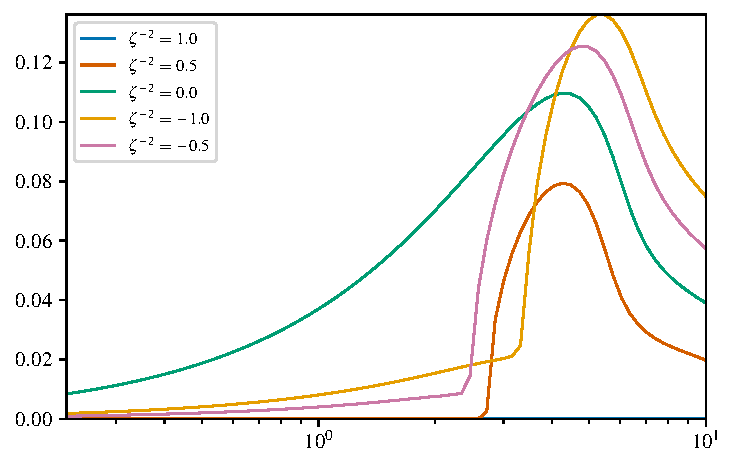
\includegraphics{Charney_evalparam}
    \caption{Growth rate of Charney instability. The $x$-axis is the zonal wavenumber.}
    \label{fig:Charney_evalparam}
\end{figure}

\subsection{Instability profiles}
We pick the two cases of $\{\xi^{-2}\}=\pm0.5$ to look at the profile of the instability. Note that $\{\xi^{-2}\}$ is eastward. Figure \ref{fig:Charney_evecmag} shows the magnitude of the eigenvector of the fastest growing mode, a common value of interest for baroclinic instability. Figure \ref{fig:Charney_instabprofile_west} and \ref{fig:Charney_instabprofile_east} shows some physical variables of the most unstable wavenumber for the westward and eastward case, respectively. We see that the streamfunctions $\psi$ and meridional velocity $v$ lean against the mean flow (note that for these two plots, we actually reserve the mean flow and keep $\beta$ unchanged). They are also out of phase, typical of baroclinic instability.

\begin{figure}
    \centering
    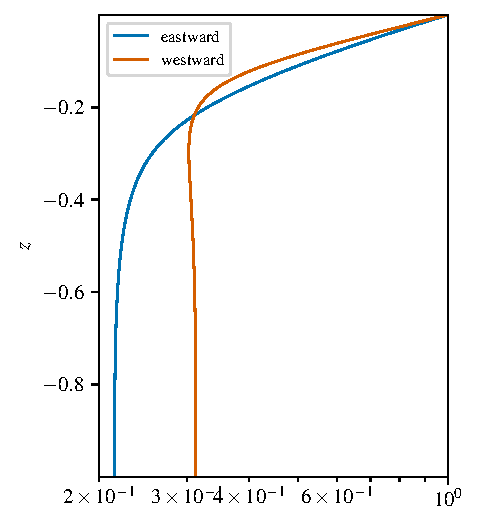
\includegraphics{Charney_evecmag}
    \caption{The magnitude of the eigenvector of the fastest growing mode.}
    \label{fig:Charney_evecmag}
\end{figure}

\begin{figure}
    \centering
    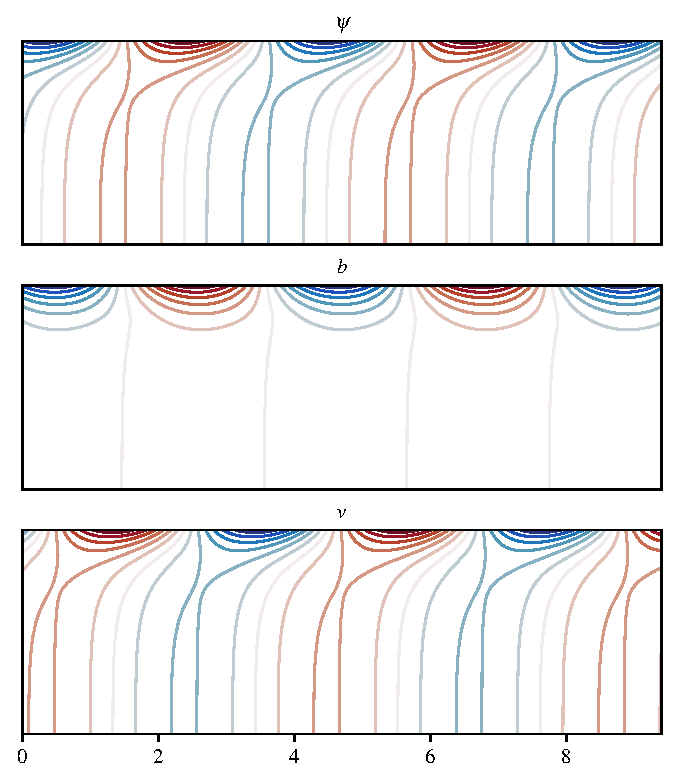
\includegraphics{Charney_instabprofile_west}
    \caption{Physical variables of the most unstable wavenumber for the westward case.}
    \label{fig:Charney_instabprofile_west}
\end{figure}

\begin{figure}
    \centering
    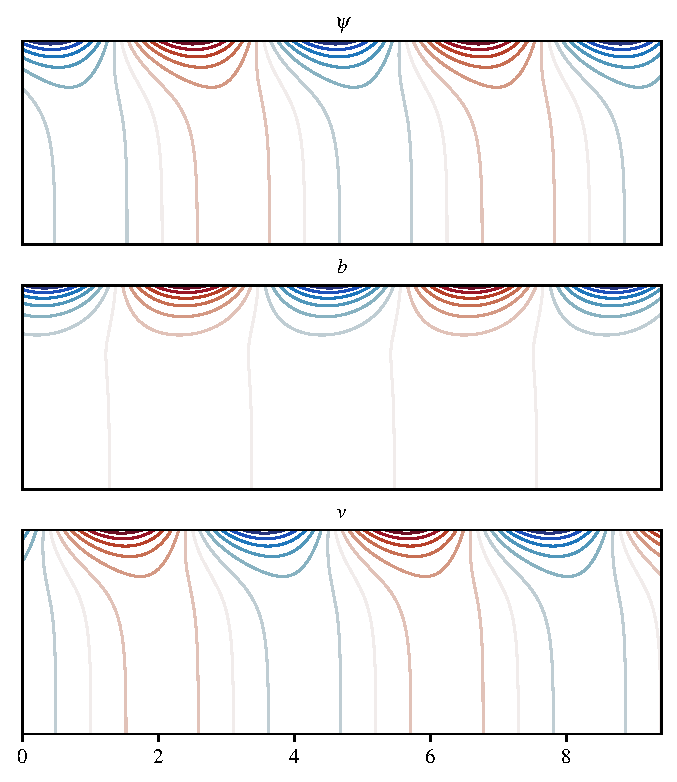
\includegraphics{Charney_instabprofile_east}
    \caption{Same as Figure \ref{fig:Charney_instabprofile_west} but for the eastward case.}
    \label{fig:Charney_instabprofile_east}
\end{figure}

\section{Some comments}
\cite{LuoCallies_23} has code to do linear instability analysis in Dedalus v2. We figured out how to obtain the eigenvectors from their code. In particular, we learned about the functions \verb|solver.set_state| and \verb|solver.state|, which exist in Dedalus v3 with modifications.




\newpage
\printbibliography

\end{document}
